\begin{frame}[c]{}

\centering
\huge
Lecture 4:\\
Hyperparameter optimization\\
Bayesian Optimization
\end{frame}
%----------------------------------------------------------------------
\begin{frame}[c]{Where are we? The big picture}

\begin{itemize}
	\item Introduction
	\item[$\to$] Background
	\begin{itemize}
		\item Design spaces in ML
		\item[$\to$] Evaluation and visualization
	\end{itemize}
	\item Hyperparameter optimization (HPO)
	\begin{itemize}
		\item Bayesian optimization
		\item Other black-box techniques
		\item Speeding up HPO with multi-fidelity optimization
	\end{itemize}
	\item Pentecost (Holiday) -- no lecture
	\item Architecture search I + II
	\item Meta-Learning
	\item Learning to learn $\&$ optimize
	\item Beyond AutoML: algorithm configuration and control
	\item Project announcement and closing
\end{itemize}

\end{frame}
%----------------------------------------------------------------------

%----------------------------------------------------------------------
\begin{frame}[c]{Learning Goals}

After this lecture, you will be able to \ldots

\begin{itemize}
  \item explain the \alert{challenges in hyperparameter optimization}
  \item efficiently optimize black box functions via \alert{Bayesian Optimization}
  \begin{itemize}
    \item discuss the advantages of different \alert{surrogate models}
    \item explain the idea of \alert{acquisition functions} to trade off exploration and exploitation
  \end{itemize}
\end{itemize}


\end{frame}
%-----------------------------------------------------------------------
\section{Hyperparameter Optimization and Black-Box Optimization}
%----------------------------------------------------------------------
\begin{frame}[c]{How to Optimize Black Box Functions?}

\centering
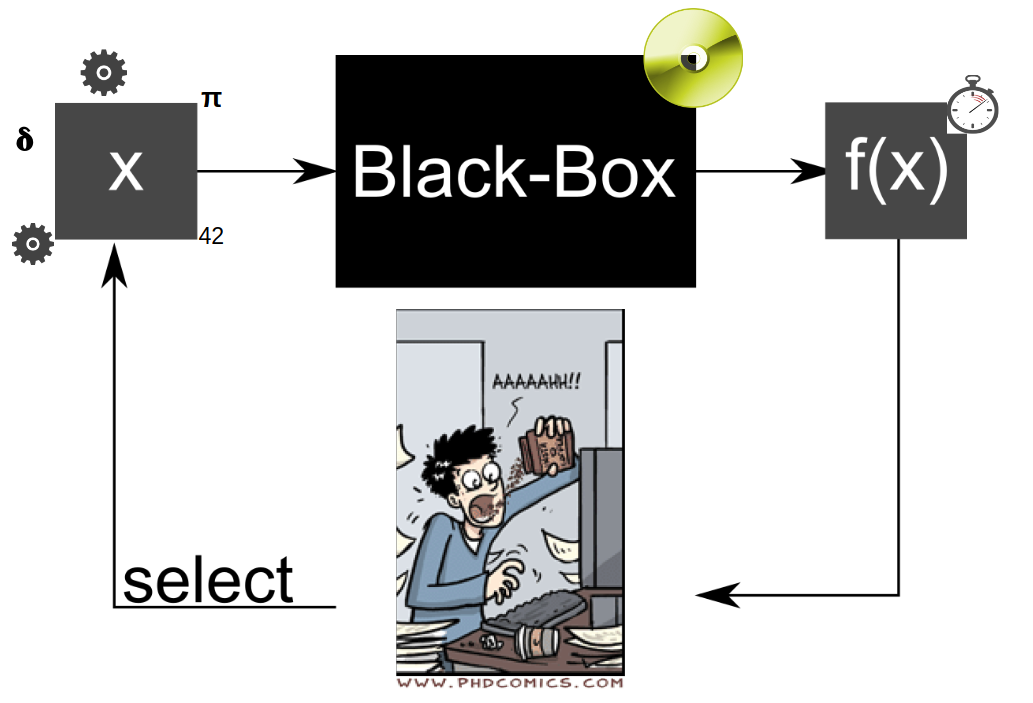
\includegraphics[width=0.7\textwidth]{images/black_box_manual_opt.png}

Only interaction: Query of function at $x$ to obtain $f(x)$

\end{frame}
%-----------------------------------------------------------------------
%----------------------------------------------------------------------
\begin{frame}[c]{How to Optimize Black Box Functions?}

\centering
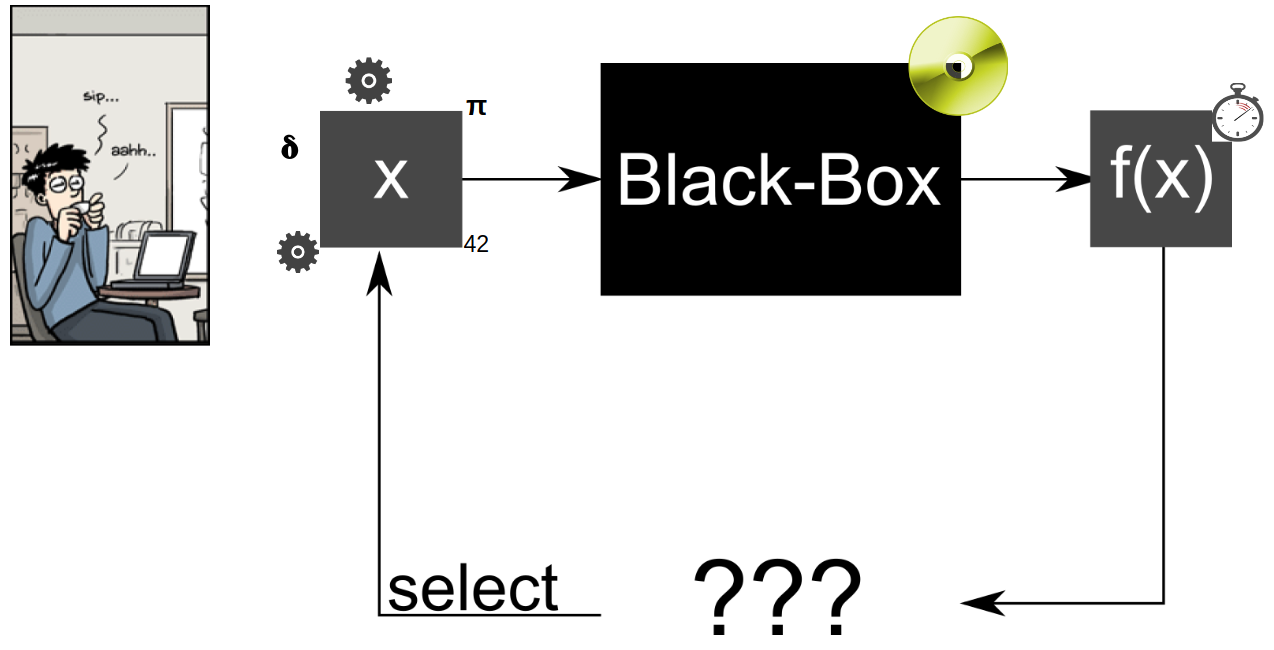
\includegraphics[width=0.9\textwidth]{images/black_box_aut_opt.png}

\end{frame}
%-----------------------------------------------------------------------
%----------------------------------------------------------------------
\begin{frame}[c]{Why Black Box Functions for AutoML?}

\begin{itemize}
  \item Internals of algorithms are often not known\\
  (or well understood)
  \item Extreme: Only way of interaction is running the algorithms
\end{itemize}

\pause
\begin{block}{Example: Hyperparameter Optimization (HPO)}
	Let 
	\begin{itemize}
		\item $\lambda$ be the hyperparameters of an ML algorithm $A$ with domain $\Lambda$,
		\item $D_{opt}$ be a training set which is split into $D_{train}$ and $D_{valid}$ 
		\item $\mathcal{L}(A_\conf, \dataset_{train}, \dataset_{valid})$ denote the loss of $A_\lambda$ trained on $D_{train}$ and evaluated on $D_{valid}$.
	\end{itemize}
	The \emph{hyper-parameter optimization (HPO)} problem is to find a hyper-parameter configuration that minimizes this loss:
	\begin{equation}
	\lambda^* \in \argmin_{\lambda \in \Lambda} \mathcal{L}(A_\conf, \dataset_{train}, \dataset_{valid}) \nonumber  
	\end{equation}
\end{block}

\end{frame}
%----------------------------------------------------------------------
%----------------------------------------------------------------------
\begin{frame}[c]{Challenges in HPO}
\only<1>
{%
	\centering
	
	\vspace*{2.25cm}
	
	What could be challenges in hyperparameter optimization? [2min]
	
	\bigskip
	
	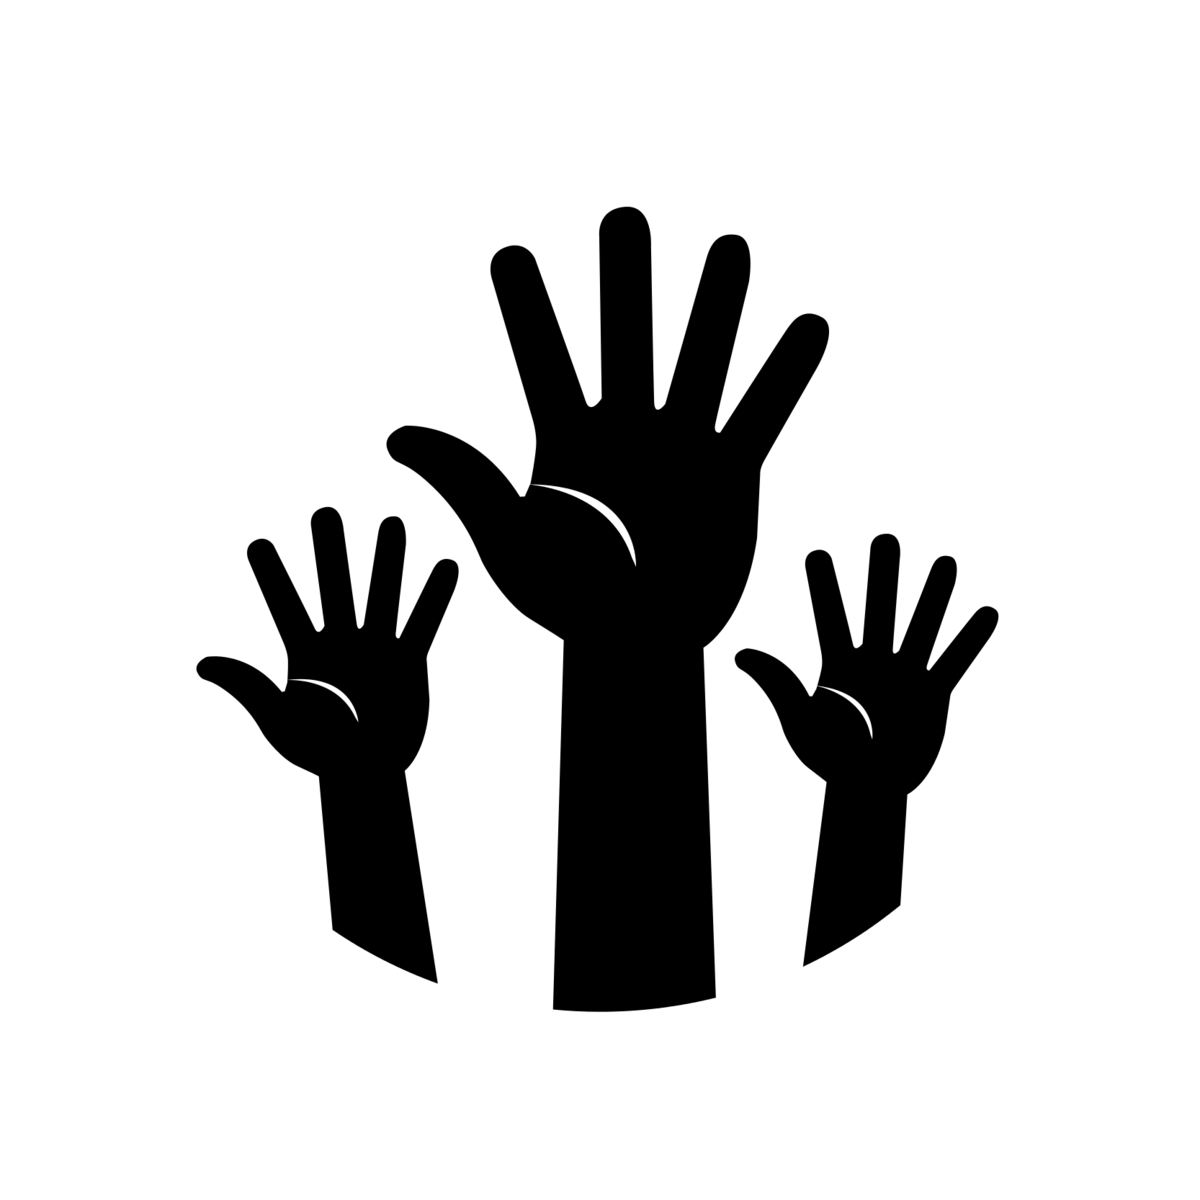
\includegraphics[width=0.2\textwidth]{images/hands.png}
}%
\pause
\begin{itemize}
  \item function evaluations are very expensive
  \begin{itemize}
    \item training a single ML-pipeline can require minutes (or even hours) 
    \item[$\leadsto$] exhaustive search is not feasible
  \end{itemize}
  \pause
  \medskip
  \item complex, structured search space
  \begin{itemize}
    \item small continuous parameter spaces already challenging to optimize
    \item typically, we talk about large configuration spaces\newline ($\gg 10$ hyper-parameters)
    \begin{itemize}
      \item many HPO benchmarks only consider a few continuous parameters
    \end{itemize}
    \item mixed parameter types
    \item conditional structures
  \end{itemize}
  \pause
  \medskip
  \item resembles a black-box optimization problem
  \begin{itemize}
    \item Input: hyperparameter configuration
    \item Black box: ML pipeline 
    \item Output: loss
    \item Note: no gradient information available
  \end{itemize}
\end{itemize}

\end{frame}
%----------------------------------------------------------------------
\begin{frame}[c]{How to Optimize Black Box Functions?}

\centering
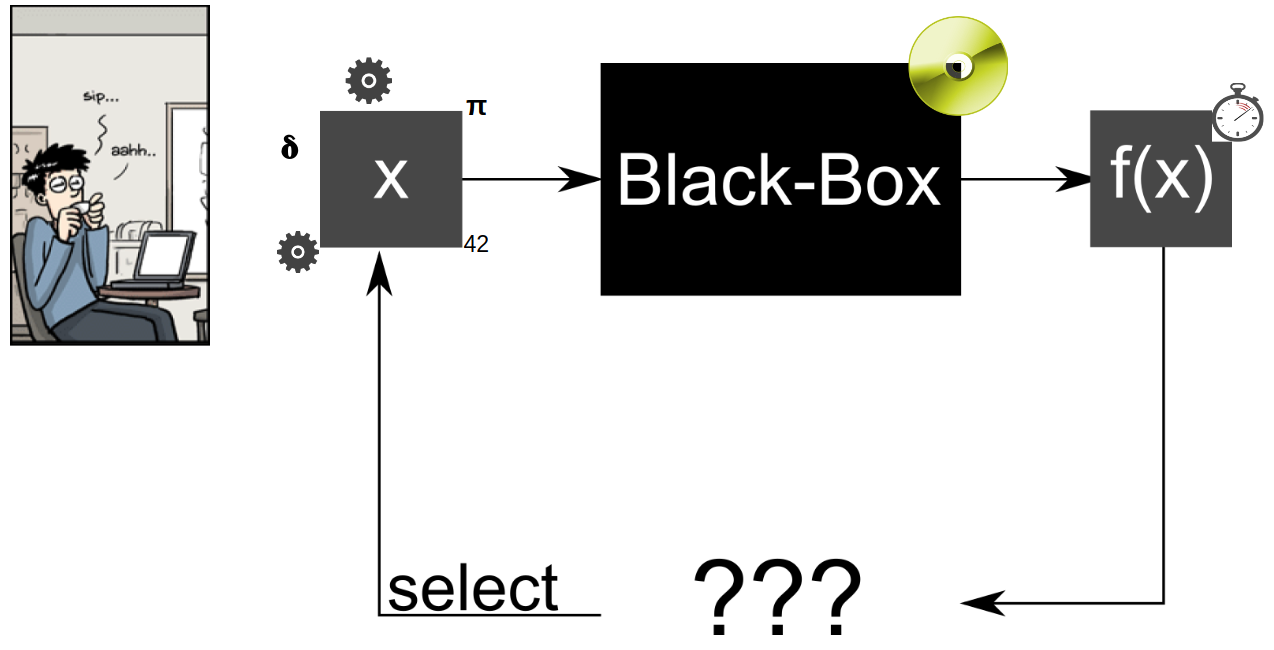
\includegraphics[width=0.9\textwidth]{images/black_box_aut_opt.png}

\end{frame}
%-----------------------------------------------------------------------
%-----------------------------------------------------------------------
\begin{frame}[c,fragile]{Grid Search \litw{Bergstra et al. '12}}

\begin{center}
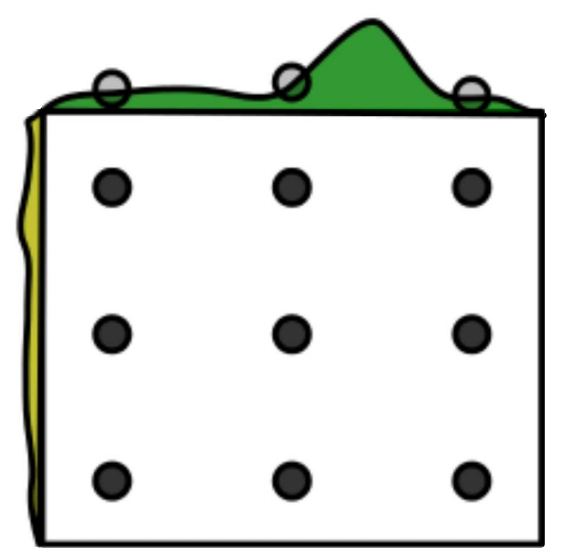
\includegraphics[width=0.28\textwidth]{images/grid_search}%
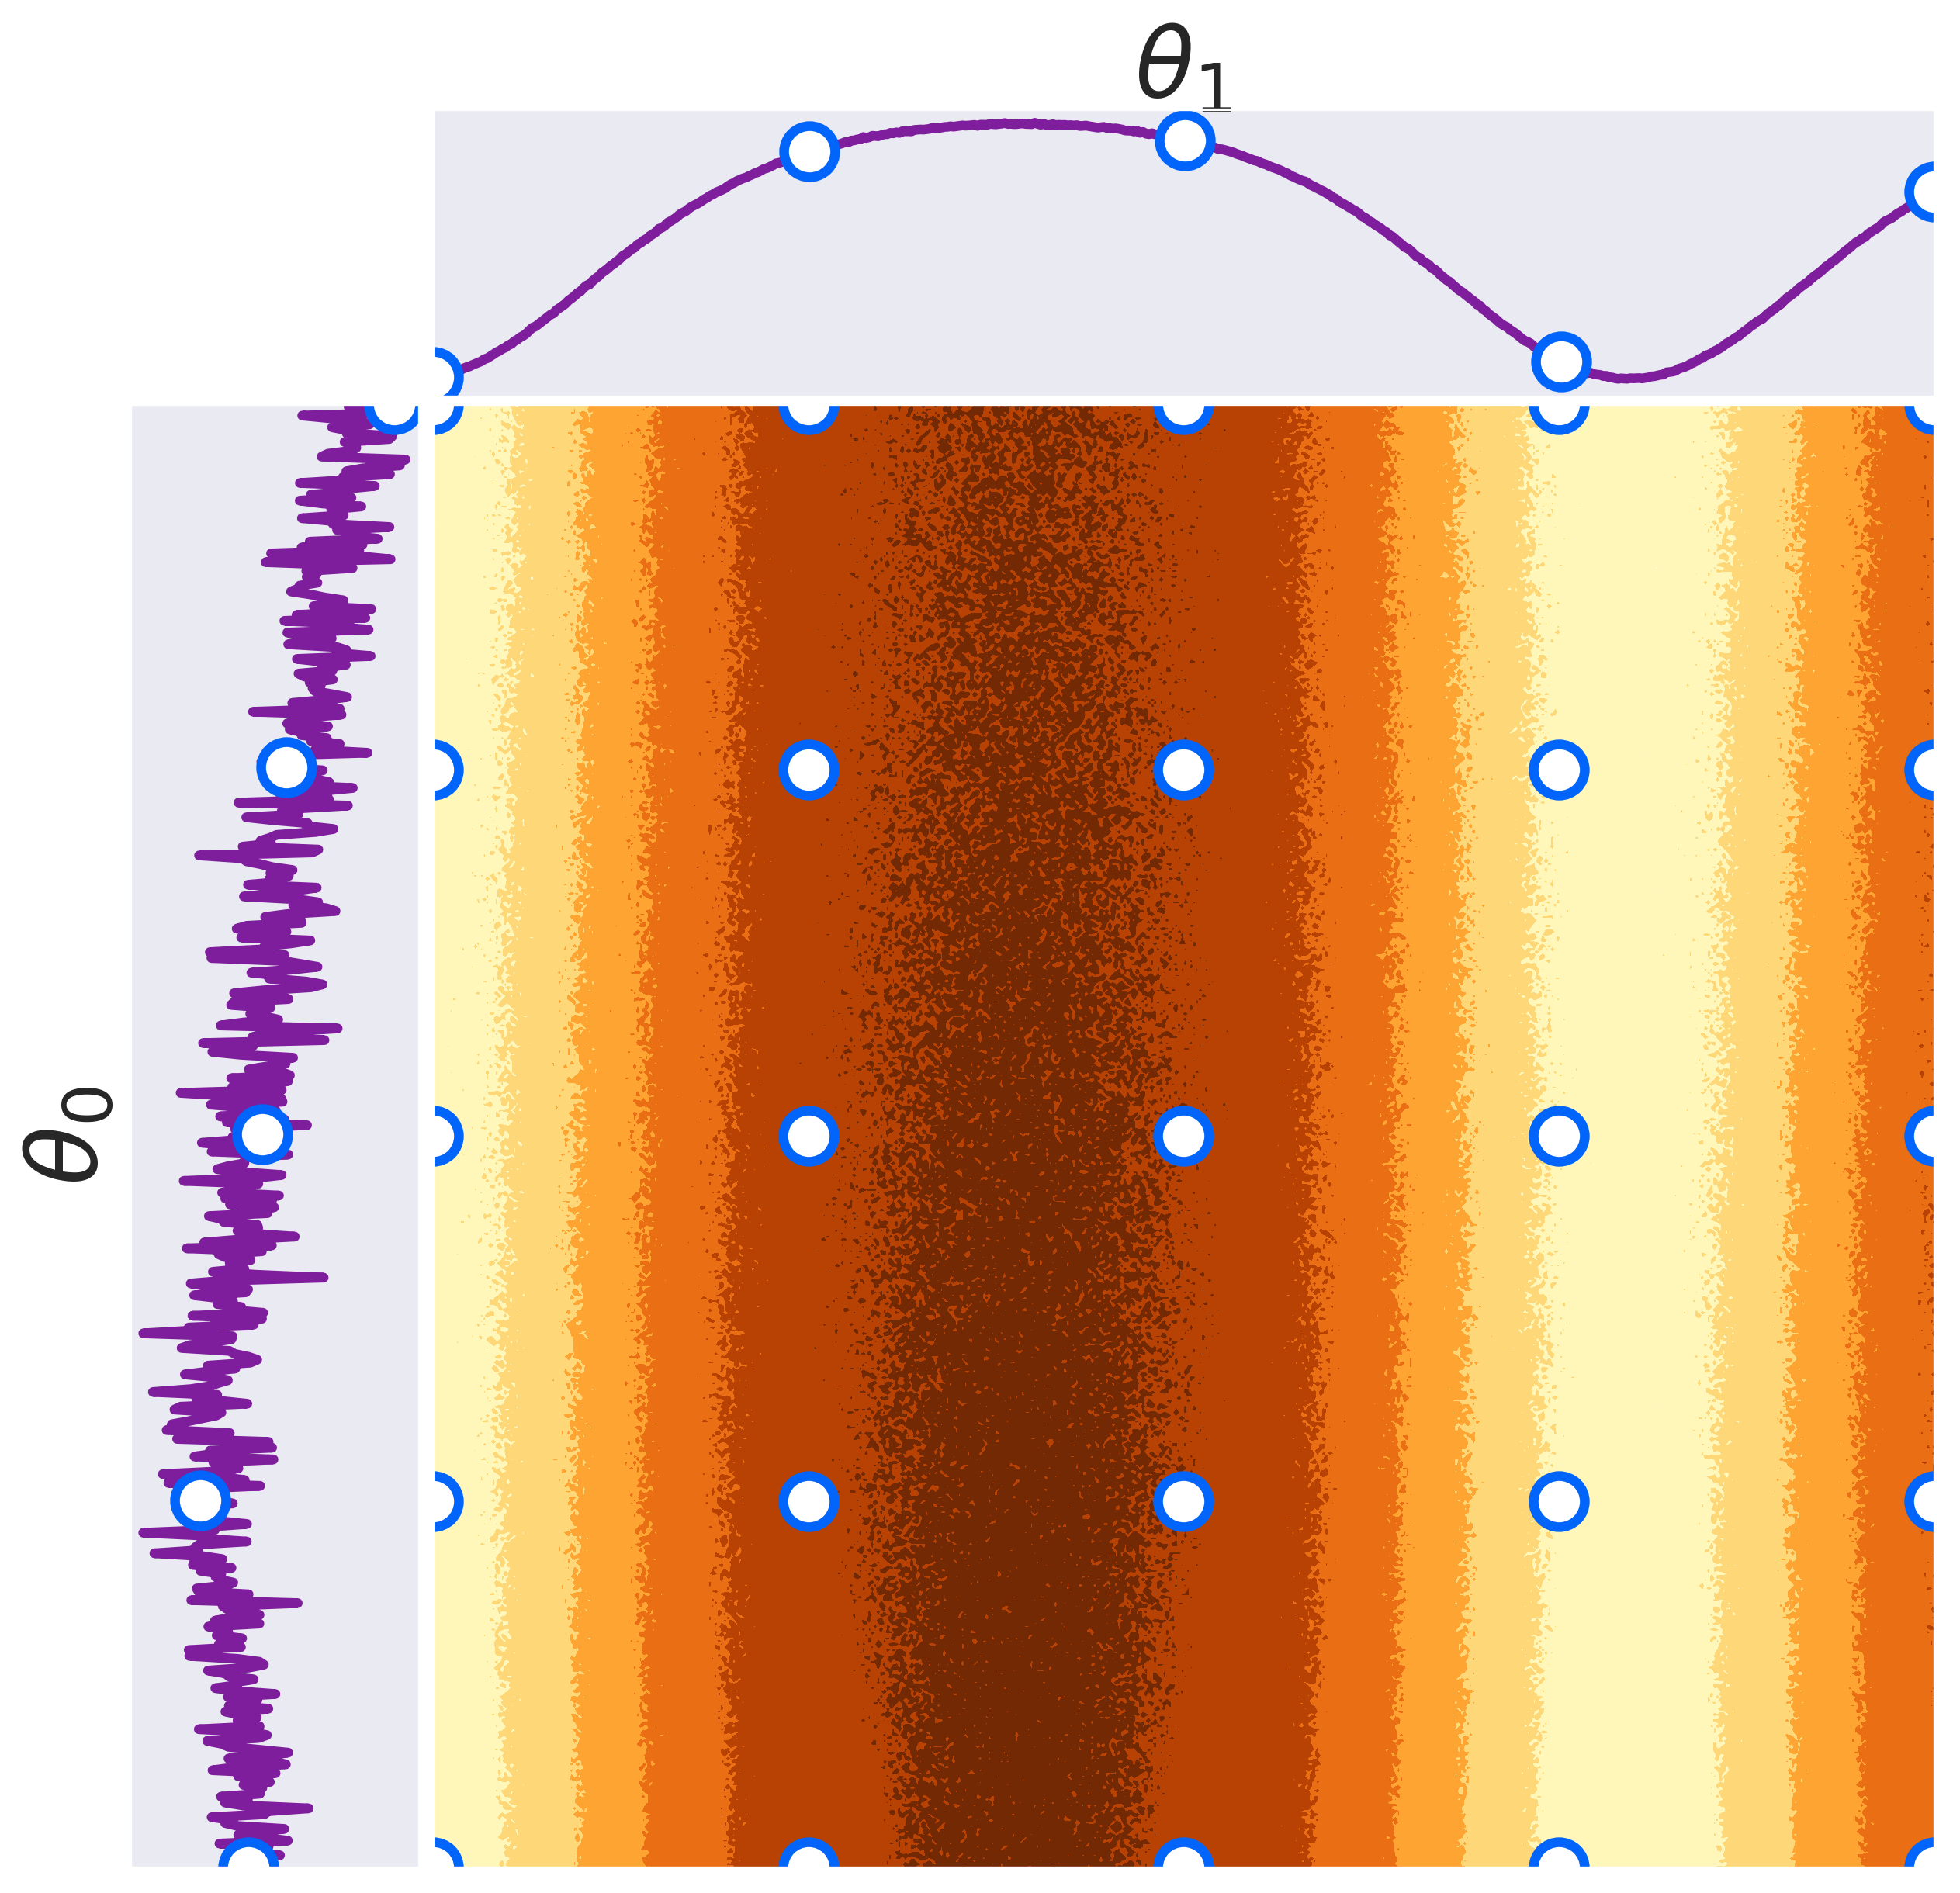
\includegraphics[width=0.28\textwidth]{images/gs}
\end{center}

\begin{block}{Pros and Cons}

\only<1-2>{\hands What are potential pros and cons of grid search?}
\pause

\begin{columns}
\column{0.4\textwidth}
Pros:
\begin{itemize}
  \item easy to implement
  \item easy to parallelize 
\end{itemize}

\column{0.6\textwidth}
Cons:
\begin{itemize}
  \item discretization of $\pcs$?
  \item does not scale with $\#$hyperparameters
  \item inefficient if not all hyperparameters are important
\end{itemize}


\end{columns}

\end{block}

\end{frame}
%-----------------------------------------------------------------------
%-----------------------------------------------------------------------
\begin{frame}[c,fragile]{Random Search \litw{Bergstra et al. '12}}

\begin{center}
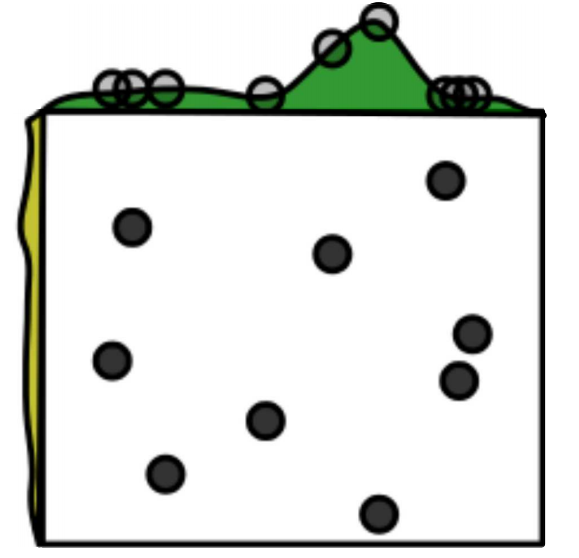
\includegraphics[width=0.28\textwidth]{images/random_search}%
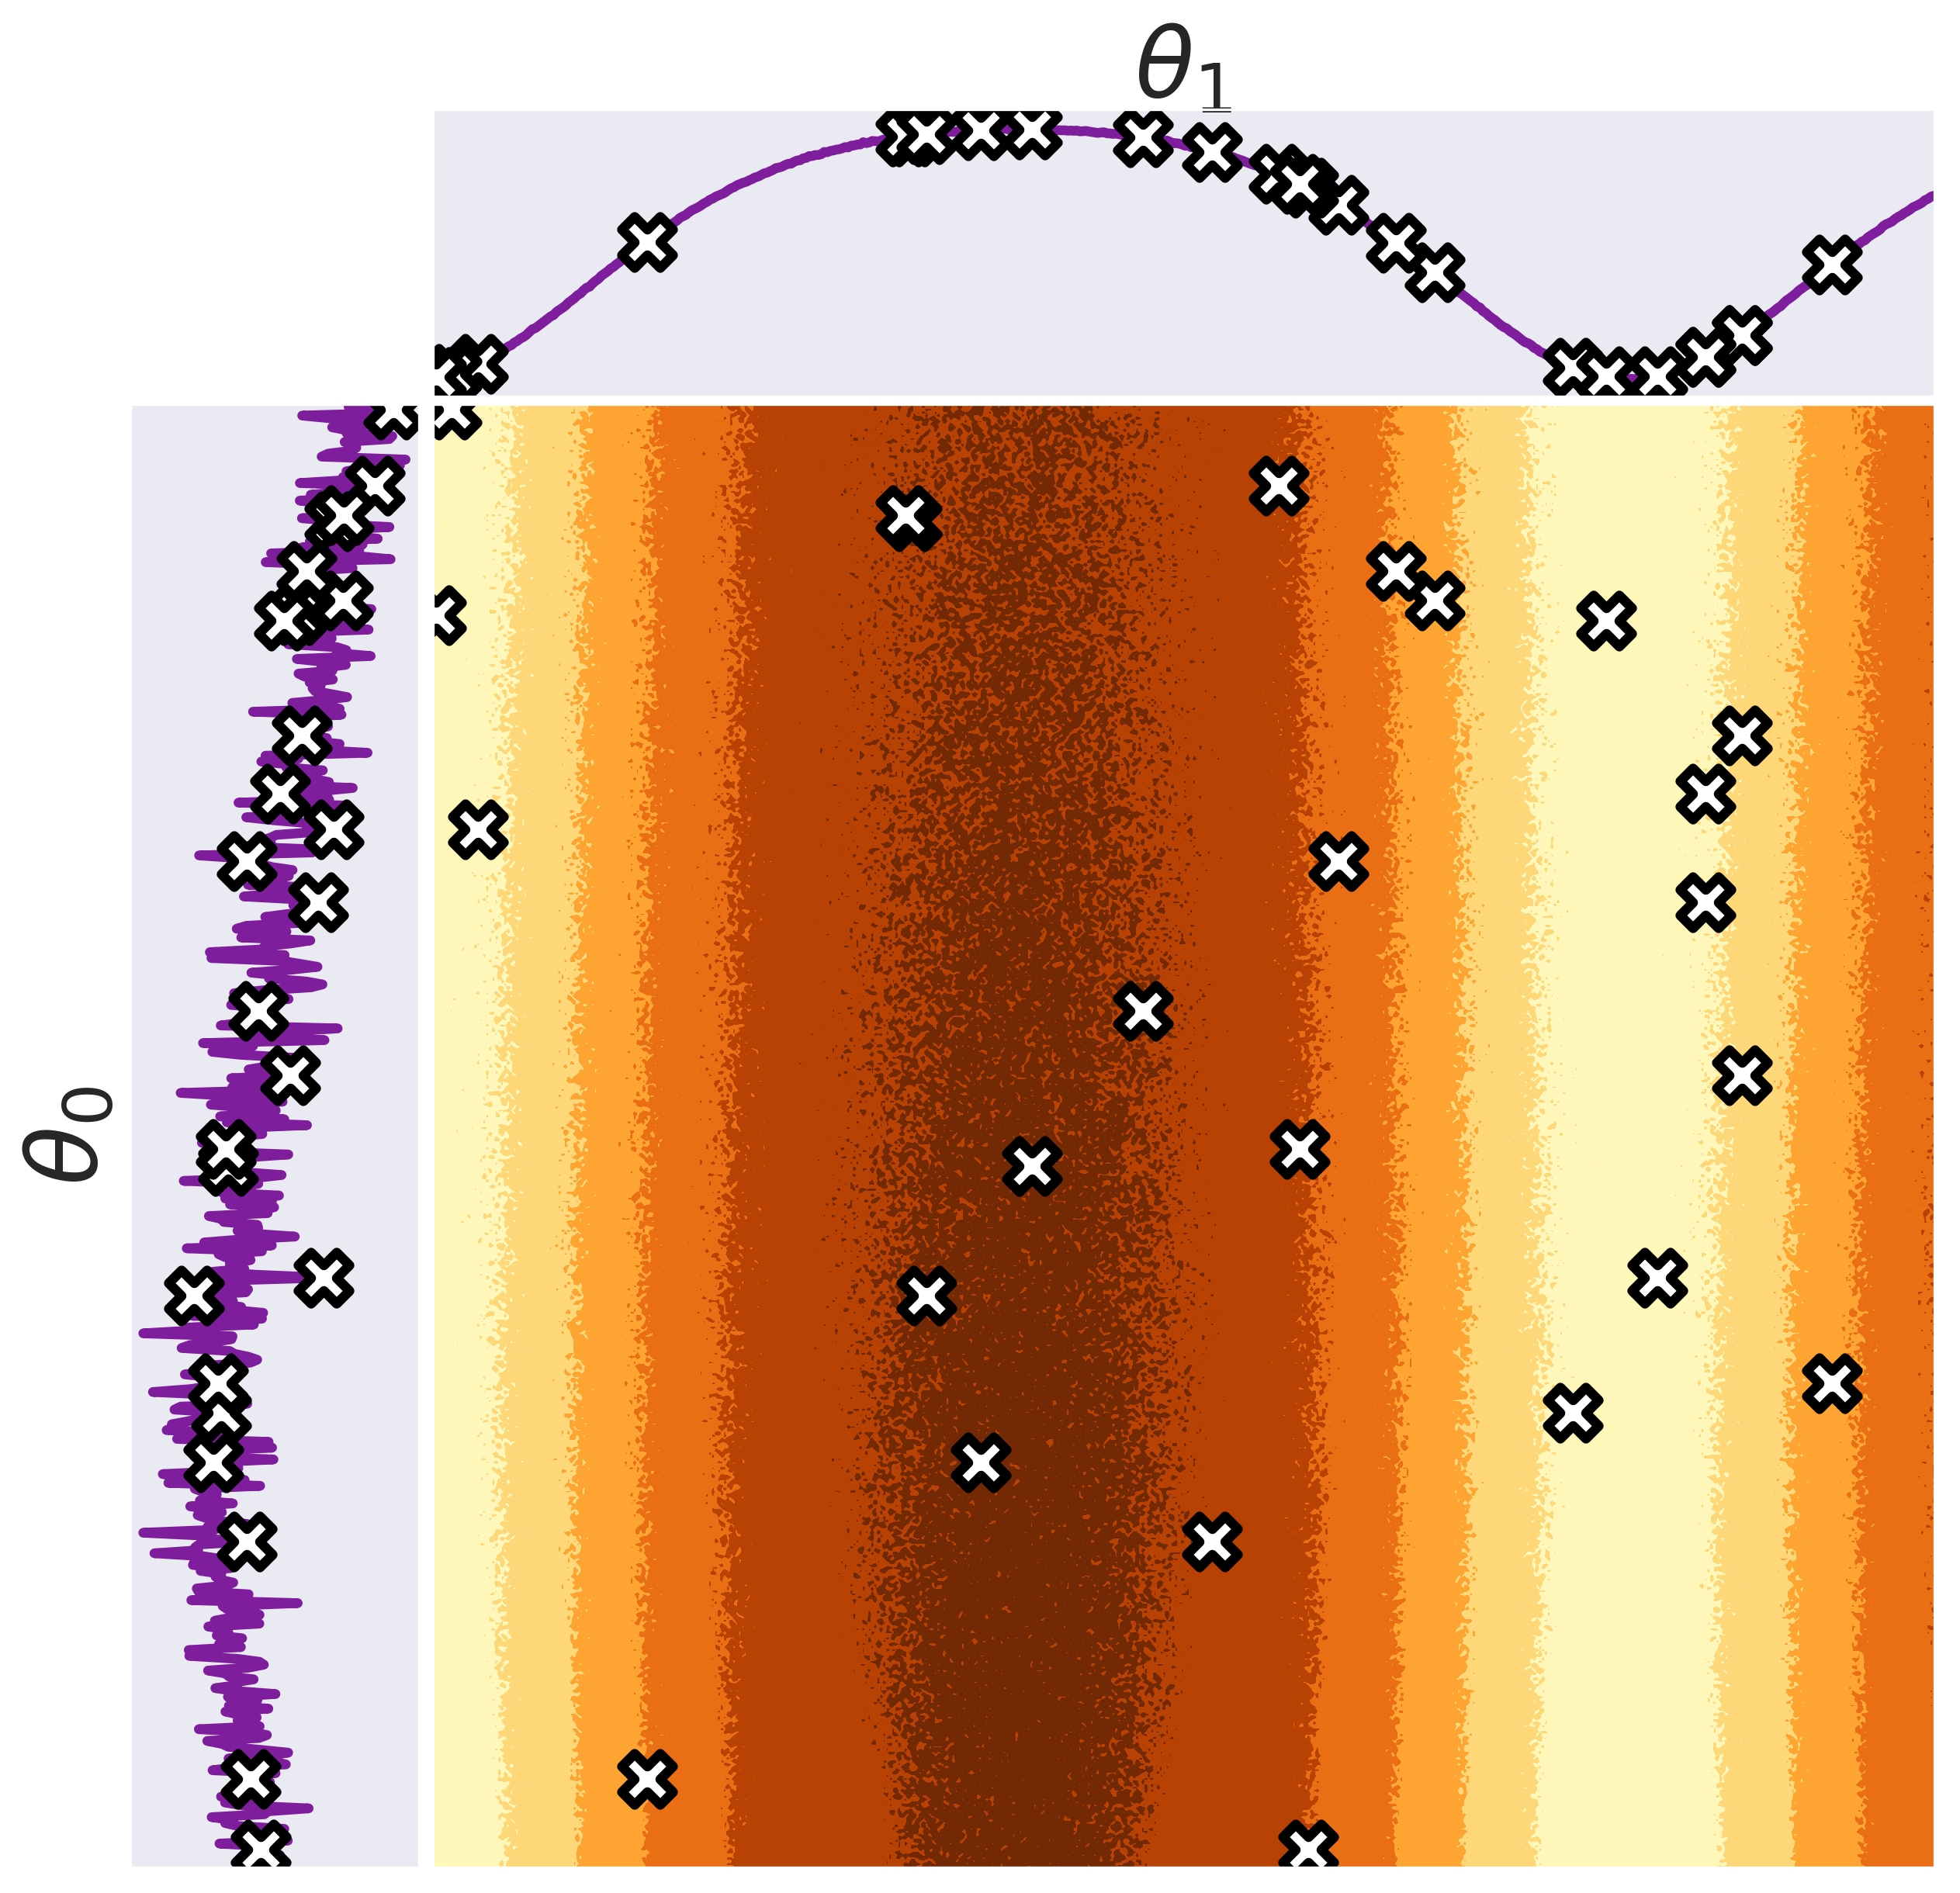
\includegraphics[width=0.28\textwidth]{images/rs}
\end{center}

\begin{block}{Pros and Cons}

\only<1-2>{\hands What are potential pros and cons of random search?}
\pause

\begin{columns}
\column{0.4\textwidth}
Pros:
\begin{itemize}
  \item even easier to implement
  \item easy to parallelize 
  \item more evaluations along each parameter
\end{itemize}

\column{0.6\textwidth}
Cons:
\begin{itemize}
  \item does not scale with $\#$hyper-parameters
  \item purely explorative
\end{itemize}


\end{columns}

\end{block}

\end{frame}
%-----------------------------------------------------------------------

%-----------------------------------------------------------------------
\begin{frame}[c,fragile]{Optimization for HPO}

\begin{itemize}
	\item HPO is expensive $\leadsto$ we need also a greedy optimization approach
	\item basically, all black-box optimization approaches could be used
	\begin{itemize}
		\item Local search
		\begin{itemize}
			\item hypothesis: HPO surfaces have many local optima s.t. local search gets easily trapped in local optima
		\end{itemize}
	 	\medskip
		\item population-based evolution strategies (more next week)
		\begin{itemize}
			\item often needs many function evaluations to perform well
		\end{itemize}
		\medskip
		\item model-based approaches
		\begin{itemize}
			\item Idea: use an surrogate model to approximate the unknown function to be optimized and do parts of the optimization on these surrogate models
		\end{itemize}
	    \item Remark: there are also combinations of these approaches (such as model-based ES)
	\end{itemize}
\end{itemize}

\end{frame}
%-----------------------------------------------------------------------
%-----------------------------------------------------------------------
\begin{frame}[c,fragile]{Black-Box Optimization: Remarks}

\begin{itemize}
	\item Expensive black-box optimization is a quite common problem in many disciplines 
	(not only limited to HPO)
	\item Examples include:
	\begin{itemize}
		\item General algorithm configuration
		\item parameter optimization of expensive simulations
		\item automatic design of experiments (e.g., in material science)
		\item tuning of robots
		\item experimental particle physics
		\item and many more ...
	\end{itemize}
	\medskip
	\pause
	\item You should consider model-based optimization approaches,\\ such as Bayesian Optimization, if ...
	\begin{enumerate}
		\item you can afford only a few function evaluations
		\item you don't care too much about the overhead induced by the optimization algorithm
	\end{enumerate}
\end{itemize}

\end{frame}
%-----------------------------------------------------------------------
\section{Tree-Parzen Estimator}
%-----------------------------------------------------------------------
\begin{frame}[c,fragile]{Tree-Parzen Estimator \litw{Bergstra et al. 2011}}

\begin{itemize}
	\item Assume that we already observed some configuration and the corresponding loss $D = \{(\conf_i, y_i))\}_{i=1}^N$
	\begin{itemize}
		\item let's use $y_i = f(\lambda)$ as a short form for $\loss(\algo_\conf, \dataset_{train}, \dataset_{valid})$
	\end{itemize}
	\pause
	\item We could approximate the good and the bad regions of the configuration space $\pcs$
\end{itemize}

$$
p(\conf|y) = \begin{cases}
l(\conf) \text{ if } y < y^*\\
g(\conf) \text{ otherwise} 
\end{cases}
$$

where 
\begin{itemize}
	\item $y^*$ is an empirical threshold for a well-performing configuration (e.g., a $\gamma$ percentile of all observed $y$ in $D$)
	\item $l(\conf)$ models the density of the well-performing region based on $D$
	\begin{itemize}
		\item Note that we minimize!
	\end{itemize}
	\item $g(\conf)$ models the density of the poorly performing region based on $D$
	\item $g$ and $l$ can be modeled by kernel density estimator (KDE)
\end{itemize}

\end{frame}
%-----------------------------------------------------------------------
%-----------------------------------------------------------------------
\begin{frame}[c,fragile]{Optimization with Tree-Parzen Estimator \litw{Bergstra et al. 2011}}

\begin{algorithm}[H]
	\Input{Configuration Space $\pcs$,
		black box function $f$,
		maximal number of function evaluations $m$,
		percentile $\gamma$
	}
	\BlankLine
	$D_0$ $\leftarrow$ initial\_design($\pcs$); \\
	\pause
	\For{n = $1, 2, \ldots m - |D_0|$}{
		$D_\text{good}, D_\text{bad}$ $\leftarrow$ Split $D_{n-1}$ into good and bad observations according to $\gamma$ percentile of all observed $y$;\\
		\pause
		$l(\conf)$ $\leftarrow$ fit KDE on $D_\text{good}$;\\
		$g(\conf)$ $\leftarrow$ fit KDE on $D_\text{bad}$;\\
		\pause
		select $\conf_{n}$ by optimizing $\conf_{n} \in \argmax_{\conf \in \pcs} l(\conf) / g(\conf)$;\\
		\pause
		Query $y_{n} := f(\lambda_{n})$;\\
		Add observation to data $D_{n} := D_{n-1} \cup \{\langle \conf_{n}, y_{n} \rangle \}$;\\
	}
	\Return{Best observed $\lambda$ according to $D_m$}
	\caption{Optimization with TPE}
\end{algorithm}


\end{frame}
%-----------------------------------------------------------------------
%-----------------------------------------------------------------------
\begin{frame}[c,fragile]{Optimization with Tree-Parzen Estimator \litw{Bergstra et al. 2011}}

\centering
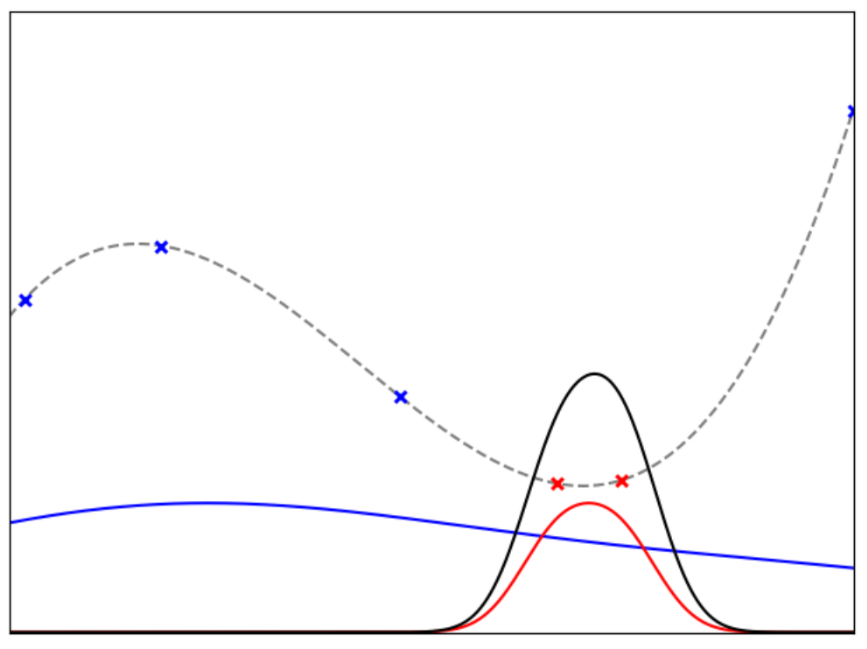
\includegraphics[width=0.8\textwidth]{images/TPE.png}


\end{frame}
%-----------------------------------------------------------------------
%-----------------------------------------------------------------------
\begin{frame}[c,fragile]{Optimization with Tree-Parzen Estimator \litw{Bergstra et al. 2011}}


Remarks:

\begin{itemize}
	\item TPE models $p(\conf | y)$
	\begin{itemize}
		\item we can multiply it with a prior to add expert knowledge
	\end{itemize}
	\smallskip
	\pause
	\item Performance of TPE depends on:
	\begin{enumerate}
		\item setting of $\gamma$ to trade-off exploration and exploitation
		\item band width of the KDEs 
	\end{enumerate}
	\pause
	\smallskip
	\item optimizing $l(\conf)/g(\conf)$ is equivalent to optimizing expected improvement as acquisition function in Bayesian Optimization\\ (more in a second)
	\pause
	\smallskip
	\item successful tool implementing TPE is HyperOpt
\end{itemize}

\end{frame}
%-----------------------------------------------------------------------
\section{Bayesian Optimization}
%-----------------------------------------------------------------------
\begin{frame}[c,fragile]{Bayesian Optimization \litw{Mockus 1977, Jones et al. 1998}}

\begin{columns}

\column{0.4\textwidth}

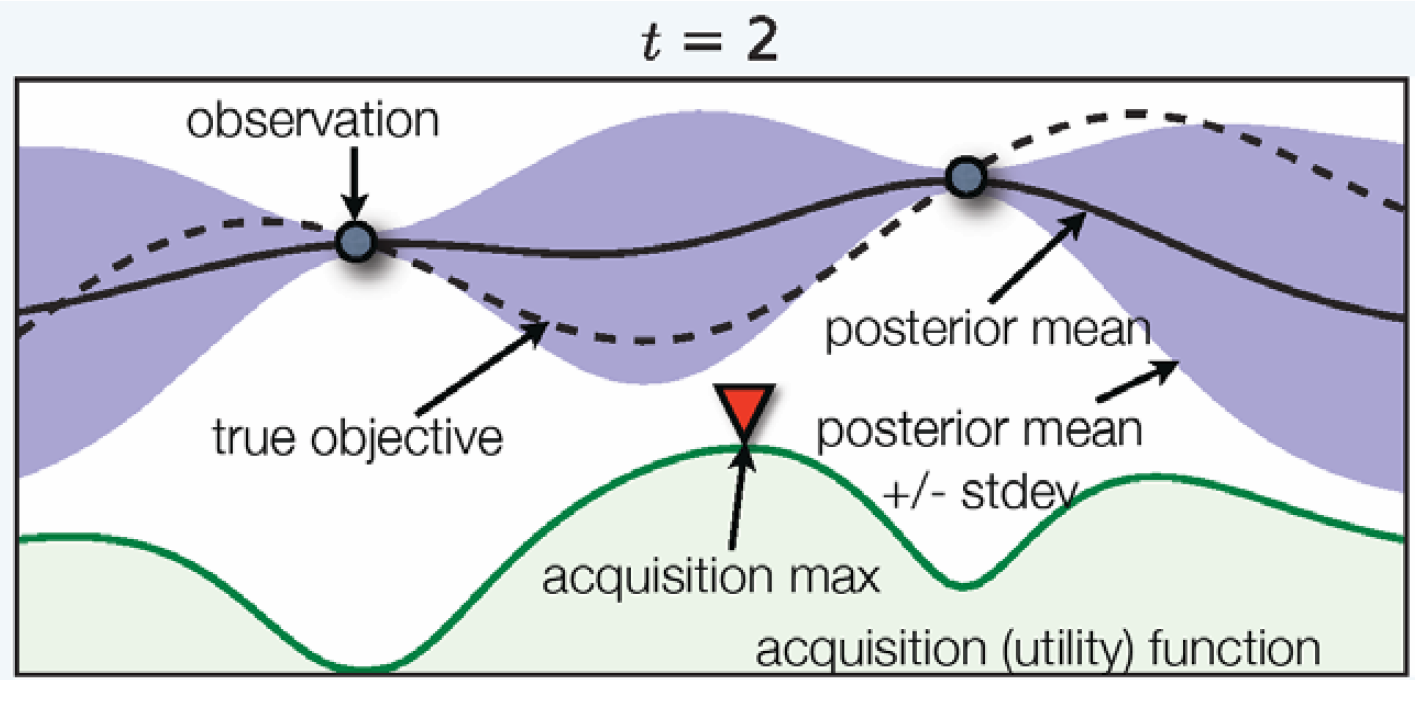
\includegraphics[width=\textwidth]{images/bo_pic1.png}\\
\pause
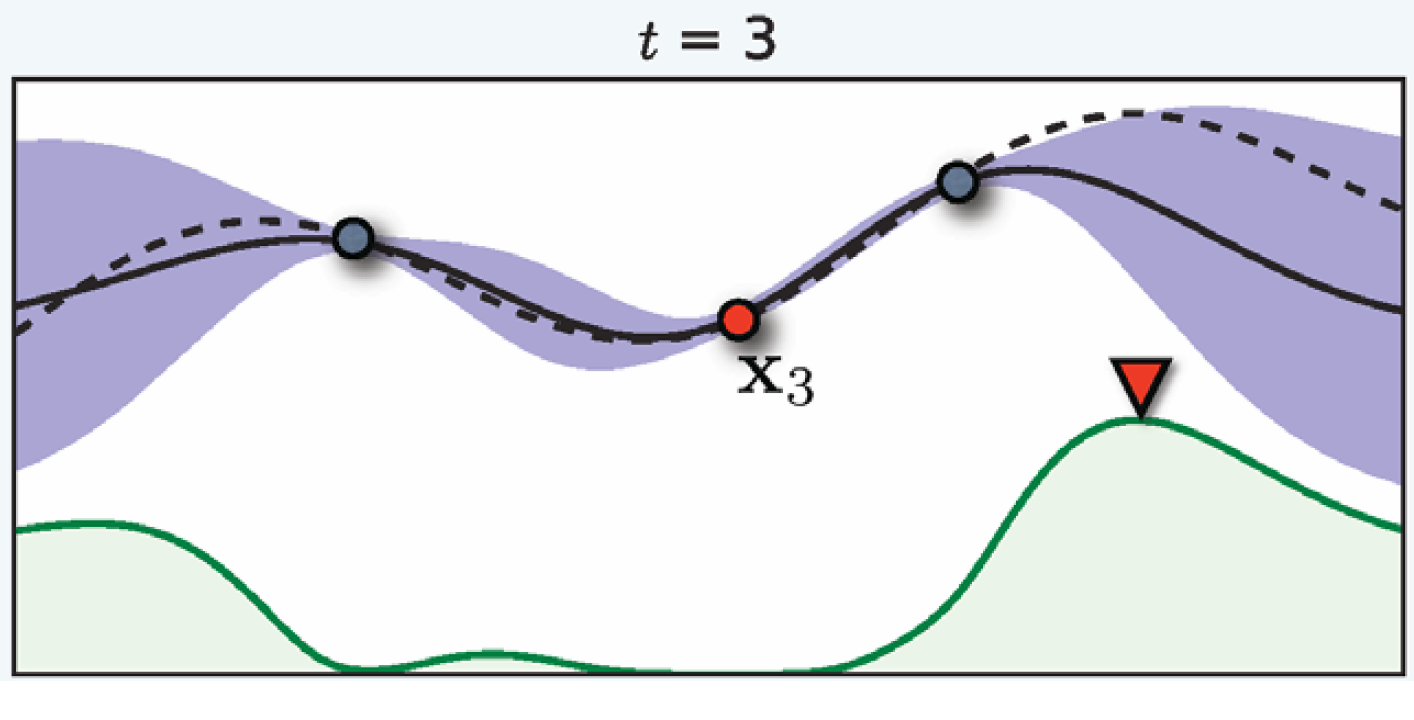
\includegraphics[width=\textwidth]{images/bo_pic2.png}\\
\pause
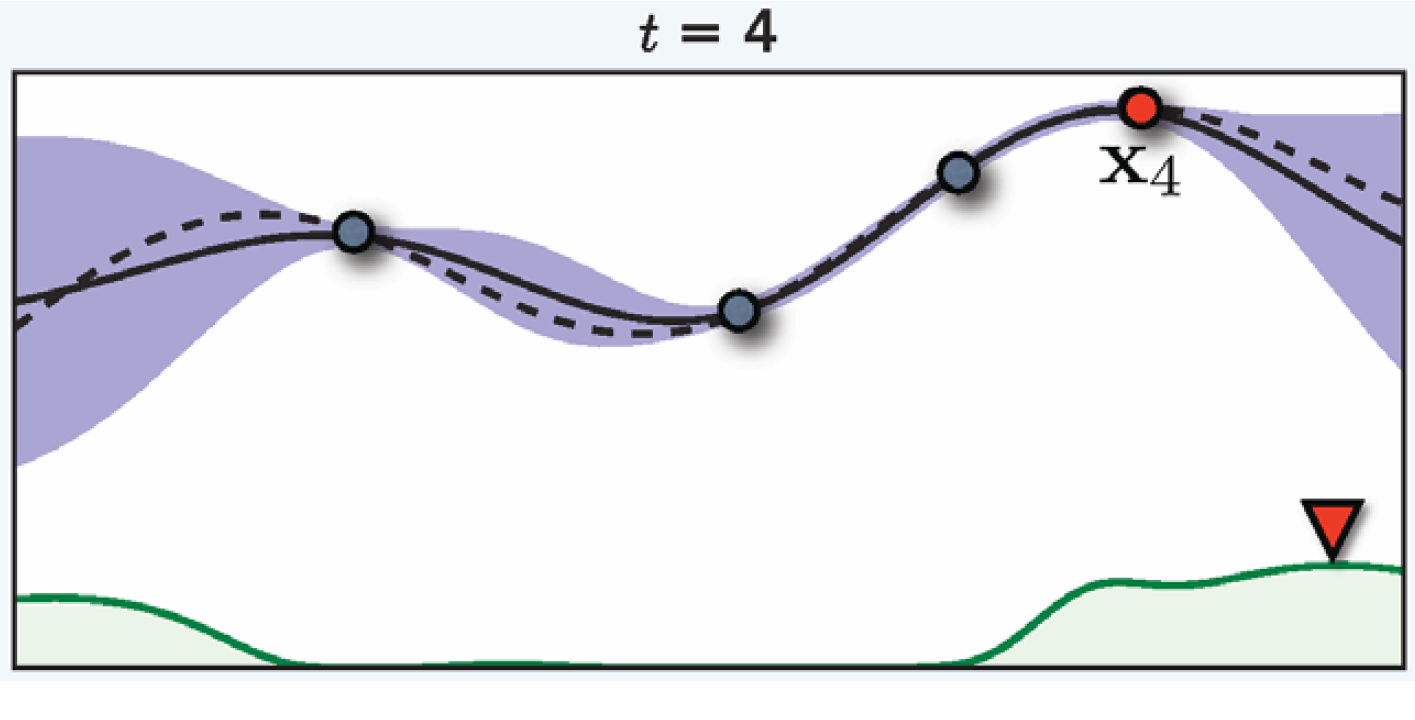
\includegraphics[width=\textwidth]{images/bo_pic3.png}
\pause

\column{0.55\textwidth}
General Approach:
\begin{enumerate}
  \item Fit model $p((f()\conf) | \conf)$ on collected observations $\langle{}\conf, f(\conf)\rangle{}$
  \pause
  \item use acquisition function $a$ to trade off exploration and exploitation
  \pause
  \item maximize acquisition function: $x^* \in \argmin a(x)$
  \pause
  \item obtain new observation at $x^*$
\end{enumerate}

\pause
Moving pieces:
\begin{itemize}
  	\item Which \alert{model family} to use 
	\item How to use the model to guide optimization
	\begin{itemize}
		\item Determined by $a(x)$\\
		(Which data point should I \emph{acquire} next?) 
	\end{itemize}
\end{itemize}

\end{columns}

\end{frame}
%-----------------------------------------------------------------------
%-----------------------------------------------------------------------
\begin{frame}[c,fragile]{Bayesian Optimization: Algorithm}

\begin{algorithm}[H]
	\Input{Search Space $\mathcal{X}$,
		black box function $f$, 
		acquisition function $\alpha$,
		maximal number of function evaluations $m$
	}
	\BlankLine
	$\mathcal{D}_0$ $\leftarrow$ initial\_design($\mathcal{X}$); \\
	\For{n = $1, 2, \ldots m - |D_0|$}{
		%\While{$B$ not exhausted} {
		$\surro: \conf \mapsto f(\lambda)$ $\leftarrow$ fit predictive model on $\mathcal{D}_{n-1}$;\\
		select $x_{n}$ by optimizing $x_{n} \in \argmax_{x \in \mathcal{X}} \alpha(x; \mathcal{D}_{n-1}, \surro)$;\\
		Query $y_{n} := f(x_{n})$;\\
		Add observation to data $D_{n} := D_{n-1} \cup \{\langle x_{n}, y_{n} \rangle \}$;\\
	}
	\Return{Best $x$ according to $D_m$ or $\surro$}
	\caption{Bayesian Optimization (BO)}
\end{algorithm}


\end{frame}
%-----------------------------------------------------------------------
%-----------------------------------------------------------------------
\begin{frame}[c,fragile]{Bayesian Optimization}

\begin{block}{Pros and Cons}

Pros:
\begin{itemize}
  \item sample efficient
  \item can be applied to many black-box functions with expensive function evaluations (not only HPO)
\end{itemize}

Cons:
\begin{itemize}
  \item overhead because of model training in each iteration
  \item hard to efficiently parallelize
  \item (requires good surrogate model)
\end{itemize}

\end{block}

\end{frame}
%-----------------------------------------------------------------------
\section{Surrogate Models}
%%%%%%%%%%%%%%%%%%%%%%%%%%%%%%%%%%%%%%%%%%%%%%%%%%%%%%%%%%%%%%%%%%%%%%%%%
\begin{frame}[c,fragile]{Surrograte Model}

Required features

\begin{itemize}
	\item Mandatory:
	\begin{itemize}
		\item Regression model
		\item Uncertainty estimates
	\end{itemize}
	\pause
	\item Preferable:
	\begin{itemize}
		\item accurate predictions
		\item cheap-to-train
		\item scales with the complexity of the data\\ (number of features and observations)
		\item can handle different types of features\\ (categorical and continuous)
	\end{itemize}
	\pause
	\medskip
	\item Candidates:
	\begin{itemize}
		\item Gaussian Processes (quite common)
		\item Random Forests (our choice)
		\item Deep Neural Networks (recent trend)
	\end{itemize}
\end{itemize}

\end{frame}
%%%%%%%%%%%%%%%%%%%%%%%%%%%%%%%%%%%%%%%%%%%%%%%%%%%%%%%%%%%%%%%%%%%%%%%%%
%%%%%%%%%%%%%%%%%%%%%%%%%%%%%%%%%%%%%%%%%%%%%%%%%%%%%%%%%%%%%%%%%%%%%%%%%
\begin{frame}[c]{Gaussian Process}

\begin{itemize}
	\item There can be several explanations (i.e., functions)\\ for a set of observations
	\item A good model would integrate over all these possible explanations (and weight them by their probability)
	\item Gaussian Processes (GPs) do exactly that by using a normal distribution assumption at each point.
\end{itemize}

\begin{block}{Informal Definition}
A Gaussian process is a collection of random variables, any finite number of which have a joint Gaussian distribution
\end{block}

\centering
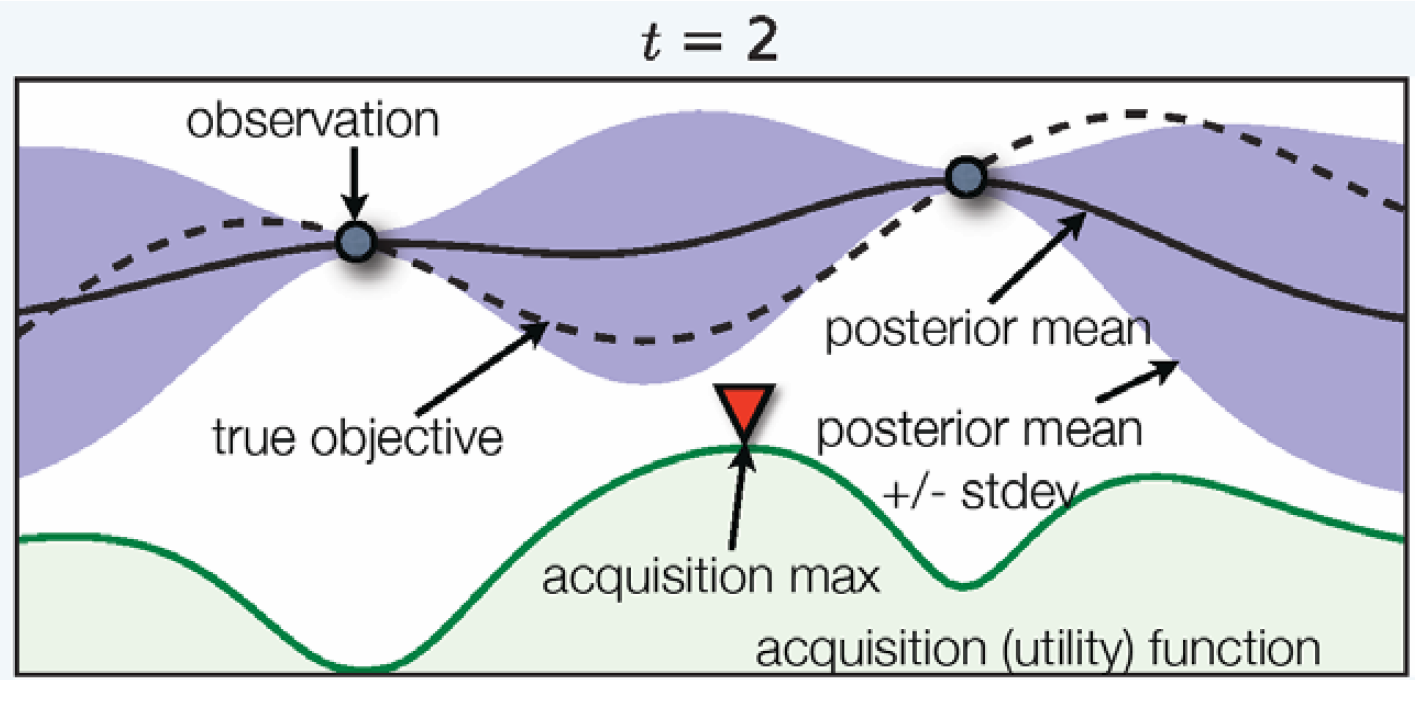
\includegraphics[width=0.5\textwidth]{images/bo_pic1.png}

\end{frame}
%%%%%%%%%%%%%%%%%%%%%%%%%%%%%%%%%%%%%%%%%%%%%%%%%%%%%%%%%%%%%%%%%%%%%%%%%
%%%%%%%%%%%%%%%%%%%%%%%%%%%%%%%%%%%%%%%%%%%%%%%%%%%%%%%%%%%%%%%%%%%%%%%%%
\begin{frame}[c]{Gaussian Process: Prior}

\centering
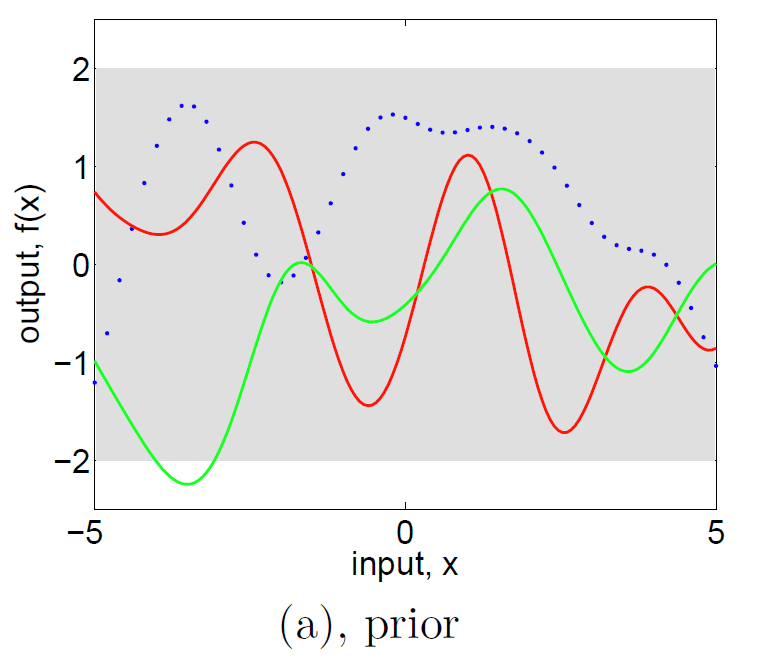
\includegraphics[width=0.5\textwidth]{images/gp_prior.png}

\begin{itemize}
	\item Samples from the prior are zero-mean, with values drawn from a multivariate Gaussian distribution $\mathcal{N}(0,\mathbf{K})$
	\item The kernel $\mathbf{K}$ tells 
	us how correlated the function values\\ at two points are
\end{itemize}

\end{frame}
%%%%%%%%%%%%%%%%%%%%%%%%%%%%%%%%%%%%%%%%%%%%%%%%%%%%%%%%%%%%%%%%%%%%%%%%%
%%%%%%%%%%%%%%%%%%%%%%%%%%%%%%%%%%%%%%%%%%%%%%%%%%%%%%%%%%%%%%%%%%%%%%%%%
\begin{frame}[c]{Gaussian Process: RBF Kernel}

\begin{equation}
k(x_i,x_j) = \exp \left(- \frac{1}{2\theta^2} || x_i - x_j ||^2 \right) \nonumber
\end{equation}

\centering
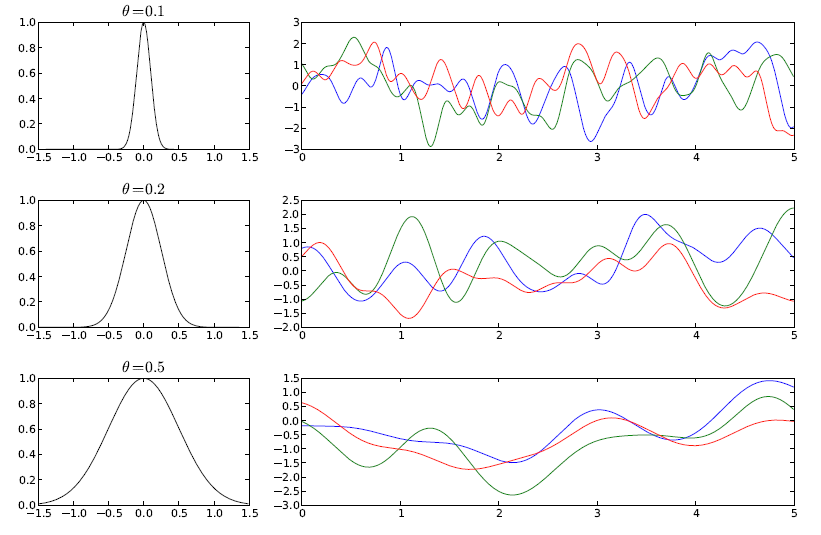
\includegraphics[width=0.8\textwidth]{images/gp_rbf_kernel.png}

\end{frame}
%%%%%%%%%%%%%%%%%%%%%%%%%%%%%%%%%%%%%%%%%%%%%%%%%%%%%%%%%%%%%%%%%%%%%%%%%
%%%%%%%%%%%%%%%%%%%%%%%%%%%%%%%%%%%%%%%%%%%%%%%%%%%%%%%%%%%%%%%%%%%%%%%%%
\begin{frame}[c]{Gaussian Process: Posterior}

\centering
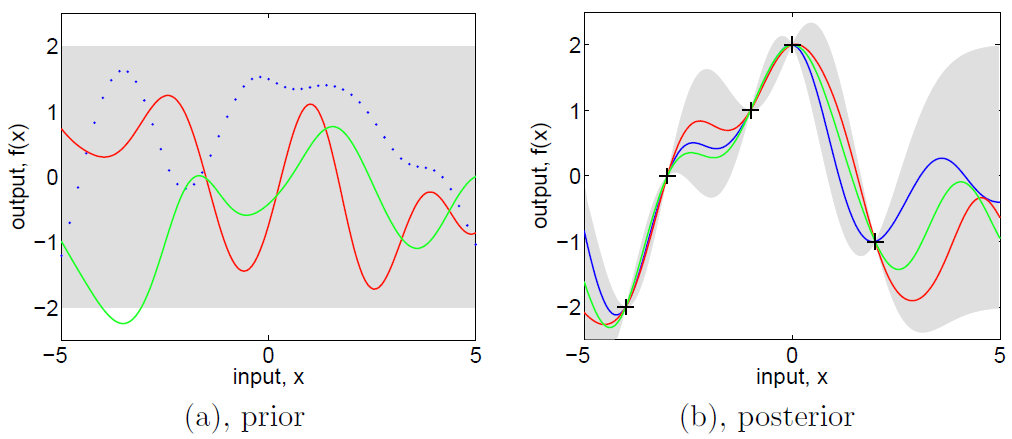
\includegraphics[width=0.9\textwidth]{images/gp_postrior.png}


\begin{eqnarray}
P(f_{t+1} | D_t, \vec{x}_{t+1})  =& \mathcal{N}(\mu_t(\vec{x}_{t+1}),\sigma_t^2(\vec{x}_{t+1})) \text{ where} \nonumber\\ 
\mu_t(\vec{x}_{t+1})  =& \mathbf{k}^T\mathbf{K}^{-1}f_{1:t} \nonumber \\ 
\sigma_t^2(\vec{x}_{t+1}) =& k(\vec{x}_{t+1},\vec{x}_{t+1}) \nonumber \mathbf{k}^T\mathbf{K}^-1\mathbf{k}
\end{eqnarray}

\end{frame}
%%%%%%%%%%%%%%%%%%%%%%%%%%%%%%%%%%%%%%%%%%%%%%%%%%%%%%%%%%%%%%%%%%%%%%%%%
%%%%%%%%%%%%%%%%%%%%%%%%%%%%%%%%%%%%%%%%%%%%%%%%%%%%%%%%%%%%%%%%%%%%%%%%%
\begin{frame}[c]{Gaussian Process: Remarks}

\begin{itemize}
	\item GPs are very good models for small-dimensional, continuous functions
	\item Advantage: we can encode in the kernel expert knowledge about the design space
	\pause
	\item Disadvantage: we have to define a good kernel for each application\\ (if we don't optimize small-dimensional, continuous functions) 
	\begin{itemize}
		 \item e.g., special kernels for categorical hyperparameters and\\ conditional dependencies
	\end{itemize}
	\smallskip
	\pause
	\item GPs have a cubic scaling with the number of observations\\ (because of inverting the kernel)
	\begin{itemize}
		\item to address this issue, there are sparse GPs\\ \lit{Snelson and Ghahramani. 2005}
	\end{itemize}
\end{itemize}

\end{frame}
%%%%%%%%%%%%%%%%%%%%%%%%%%%%%%%%%%%%%%%%%%%%%%%%%%%%%%%%%%%%%%%%%%%%%%%%%
%%%%%%%%%%%%%%%%%%%%%%%%%%%%%%%%%%%%%%%%%%%%%%%%%%%%%%%%%%%%%%%%%%%%%%%%%
\begin{frame}[c,fragile]{Random Forests as Surrogate Models}


\centering
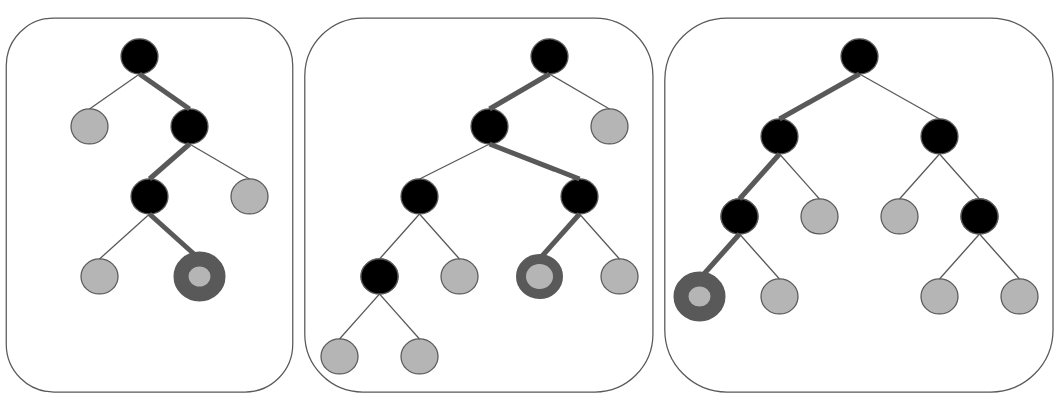
\includegraphics[width=0.55\textwidth]{images/random_forest_pic}

\begin{itemize}
\item Train:
\begin{itemize}
	\item $n$ decision (or regression) trees
	\item subsampled training data for each tree (with bootstrapping)
	\item (subsampled feature set for each split)
	\pause
	\item[$\leadsto$] each tree gives us a possible explanation for the observations
\end{itemize}

\pause

\item Predict
\begin{itemize}
	\item Obtain prediction of each tree
	\item Aggregate predictions (e.g., average)
	\pause
	\item Uncertainty of predictions: stdev across tree predictions 
\end{itemize}
\end{itemize}


\end{frame}
%%%%%%%%%%%%%%%%%%%%%%%%%%%%%%%%%%%%%%%%%%%%%%%%%%%%%%%%%%%%%%%%%%%%%%%%%
%%%%%%%%%%%%%%%%%%%%%%%%%%%%%%%%%%%%%%%%%%%%%%%%%%%%%%%%%%%%%%%%%%%%%%%%%
\begin{frame}[c,fragile]{Advantages and Disadvantages of Random Forests}


\begin{columns}
\column{0.5\textwidth}
Pros:
\begin{itemize}
\item Cheap to train
\item Scales well with \#observations
\begin{itemize}
	\item Worst-case complexity for $T$ tress with $n$ data points of dimensionality $p$: $\mathcal O(T\cdot p \cdot n^2 \log{n})$
\end{itemize}
\item training can be parallelized
\item Can handle continuous and categorical features
\begin{itemize}
	\item most RF implementations can handle only continuous features
\end{itemize}
\end{itemize}

\column{0.5\textwidth}
Cons:
\begin{itemize}
\item Poor uncertainty estimates
\item No extrapolation
\begin{itemize}
	\item last seen value for extrapolation (constant)
	\item no prior
\end{itemize}
\end{itemize}

\end{columns}

\end{frame}
%%%%%%%%%%%%%%%%%%%%%%%%%%%%%%%%%%%%%%%%%%%%%%%%%%%%%%%%%%%%%%%%%%%%%%%%%
%%%%%%%%%%%%%%%%%%%%%%%%%%%%%%%%%%%%%%%%%%%%%%%%%%%%%%%%%%%%%%%%%%%%%%%%%
\begin{frame}[c,fragile]{Deep Neural Networks as Surrogate Models}

\begin{itemize}
	\item DNNs are known to have good predictions given big data
	\item In Bayesian Optimization (BO), we have (often) little data
	\item DNNs are not known for very good uncertainty estimates
	\item Nevertheless, we can use DNN for BO
\end{itemize}

\centering
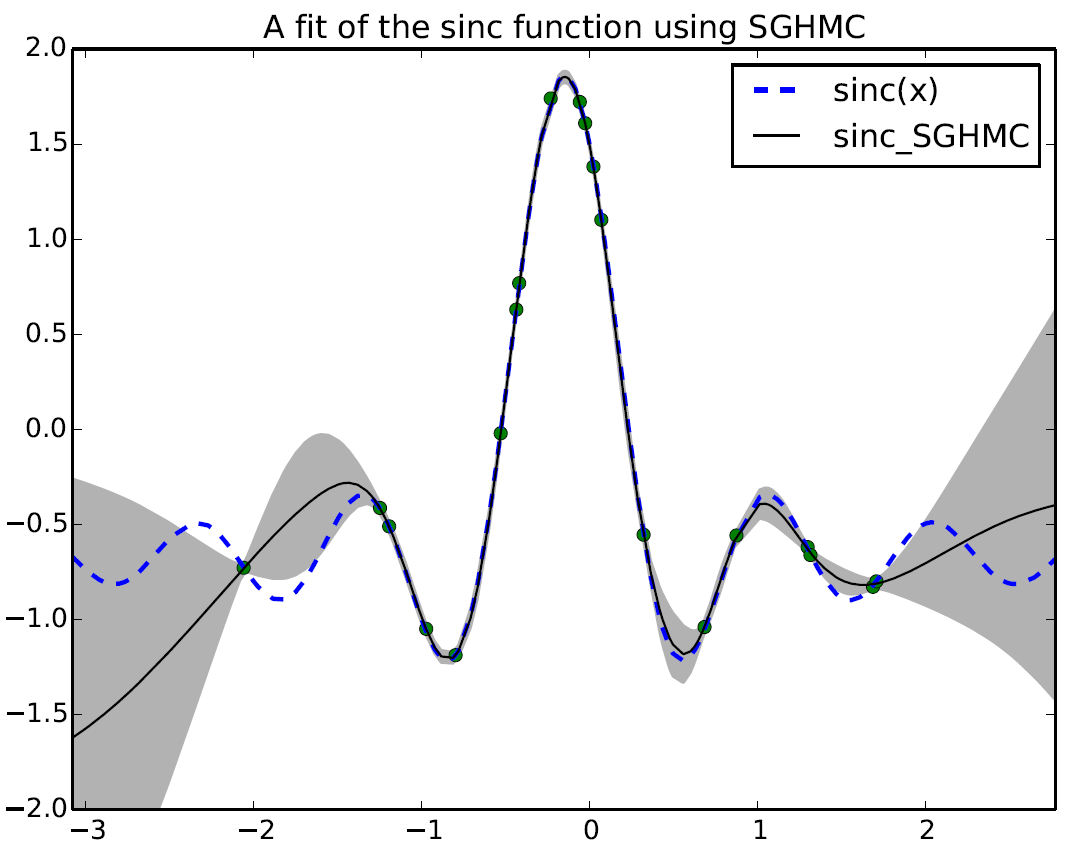
\includegraphics[width=0.5\textwidth]{images/bo_dnn.png}
\begin{flushright}
	Source: \lit{Springerberger et al. 2016}
\end{flushright}


\end{frame}
%%%%%%%%%%%%%%%%%%%%%%%%%%%%%%%%%%%%%%%%%%%%%%%%%%%%%%%%%%%%%%%%%%%%%%%%%

%%%%%%%%%%%%%%%%%%%%%%%%%%%%%%%%%%%%%%%%%%%%%%%%%%%%%%%%%%%%%%%%%%%%%%%%%
\begin{frame}[c,fragile]{DNGO~\litw{Snoek et al. 2015}}

\begin{itemize}
	\item Main idea: combine DNN with a Bayesian linear regression
	\smallskip 
	\pause
	\item 1st step: Train a DNN with linear regression as last layer to get an embedding $\phi(x)$
	\smallskip
	\pause
	\item Replace last layer by Bayesian linear regressor
	\begin{itemize}
		\item Bayesian linear regression has two hyperparameters $\alpha$, $\beta$ 
		\item Snoek et al. used slice sampling to integrate these out
	\end{itemize}
	\pause
	\item DNGO scales much better than GPs: 
\end{itemize}

\centering
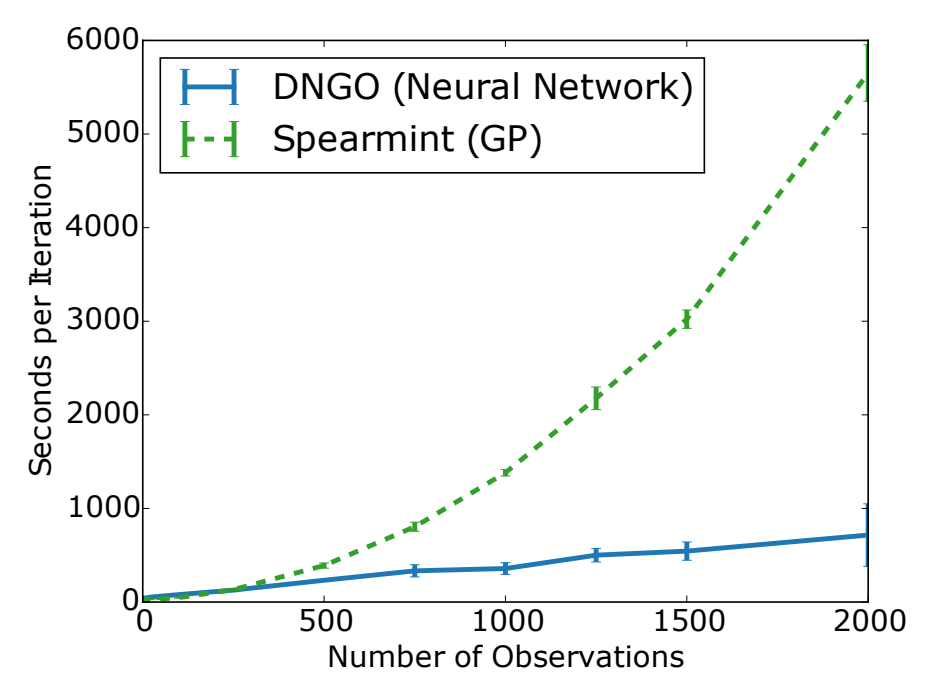
\includegraphics[width=0.5\textwidth]{images/dngo_scaling.png}
\begin{flushright}
	source: \lit{Snoek et al. 2015}
\end{flushright}

\end{frame}
%%%%%%%%%%%%%%%%%%%%%%%%%%%%%%%%%%%%%%%%%%%%%%%%%%%%%%%%%%%%%%%%%%%%%%%%%
%%%%%%%%%%%%%%%%%%%%%%%%%%%%%%%%%%%%%%%%%%%%%%%%%%%%%%%%%%%%%%%%%%%%%%%%%
\begin{frame}[c,fragile]{DNGO: Meta-Design Decisions~\litw{Snoek et al. 2015}}

\centering
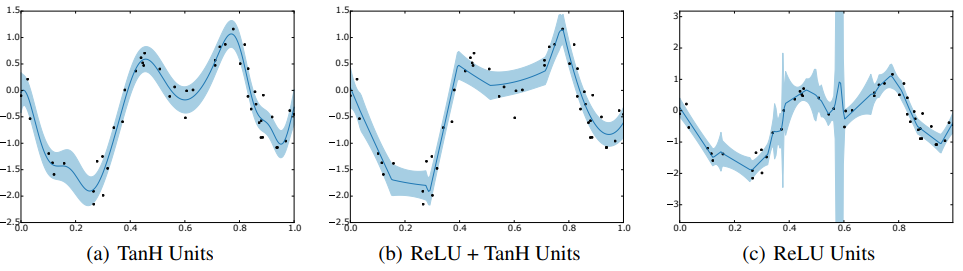
\includegraphics[width=0.9\textwidth]{images/dngo_activation.png}

\begin{itemize}
	\item the activation function is quite important to get good uncertainty estimates
	\item other hyperparameters (such as the architecture of the DNN) are also crucial
	\begin{itemize}
		\item Snoek et al. used BO to optimize these hyperparameters (as a meta-meta problem)
		\item however, the impact of this meta-meta tuning is unknown
	\end{itemize}
\end{itemize}

\end{frame}
%%%%%%%%%%%%%%%%%%%%%%%%%%%%%%%%%%%%%%%%%%%%%%%%%%%%%%%%%%%%%%%%%%%%%%%%%

%%%%%%%%%%%%%%%%%%%%%%%%%%%%%%%%%%%%%%%%%%%%%%%%%%%%%%%%%%%%%%%%%%%%%%%%%
\begin{frame}[c,fragile]{Further approaches for BO with DNNs}

\begin{itemize}
	\item \lit{Springenberger et al. 2016} proposed  Bayesian Optimization with Hamiltonian Monte Carlo Artificial Neural
	Networks (BOHAMIANN) 
	\begin{itemize}
		\item uses stochastic gradient	Hamiltonian Monte Carlo (SGHMC) for a truly Bayesian approach 
	\end{itemize}
	\medskip
	\pause
	\item \lit{Lu et al. 2018} proposed to use structured variationally auto-encoders
	\begin{enumerate}
		\item learn an embedding into a small-dimensional latent space
		\item the latent representation is fed into a GP
	\end{enumerate}
\end{itemize}

\end{frame}

%%%%%%%%%%%%%%%%%%%%%%%%%%%%%%%%%%%%%%%%%%%%%%%%%%%%%%%%%%%%%%%%%%%%%%%%%
%%%%%%%%%%%%%%%%%%%%%%%%%%%%%%%%%%%%%%%%%%%%%%%%%%%%%%%%%%%%%%%%%%%%%%%%%
\section{Acquisition Functions}
%%%%%%%%%%%%%%%%%%%%%%%%%%%%%%%%%%%%%%%%%%%%%%%%%%%%%%%%%%%%%%%%%%%%%%%%%
%%%%%%%%%%%%%%%%%%%%%%%%%%%%%%%%%%%%%%%%%%%%%%%%%%%%%%%%%%%%%%%%%%%%%%%%%

\begin{frame}[c,fragile]{The Role of the Acquisition Function}
\begin{itemize}
  \item Given: a model $\hat{f}:\confs \rightarrow \mathds{R}$ that predicts the quality $\mu(\conf)$ for each configuration $\conf$ and its standard deviation $\sigma(\conf)$ ($\leadsto$ uncertainty)
  \begin{itemize}
  	\item Assume w.l.o.g. that we want to \emph{maximize} $f$
  \end{itemize}
  \medskip
  \pause
  \item Which configuration should we select next? Need to trade off: 
  \begin{itemize}
    \item \alert{Exploitation}\\(sampling where the predicted mean $\mu(\conf)$ is high)
    \item \alert{Exploration}\\(sampling where we're uncertain about f; i.e., $\sigma(\conf)$ is high)
  \end{itemize}
  \medskip
  \pause
  \item Various acquisition functions achieve this trade-off
\end{itemize}

\end{frame}
%%%%%%%%%%%%%%%%%%%%%%%%%%%%%%%%%%%%%%%%%%%%%%%%%%%%%%%%%%%%%%%%%%%%%%%%%


%%%%%%%%%%%%%%%%%%%%%%%%%%%%%%%%%%%%%%%%%%%%%%%%%%%%%%%%%%%%%%%%%%%%%%%%%
\begin{frame}[c,fragile]{Probability of Improvement}
\begin{itemize}
\vspace*{-0.2cm}
  \item Let $f(\theta^+)$ denote the best (here: max) function value known so far.
\vspace*{-0.2cm}  
  \begin{eqnarray}
\nonumber{}  PI(\conf) & = & P(f(\conf) \ge f(\theta^+))) = \Phi \left( \frac{\mu(\theta) - f(\theta^+)}{\sigma(\theta)} \right)
  \end{eqnarray}
  \item Here, $\Phi$ is the cumulative distribution function of the standard normal distribution. (There are $\mathcal{O}(1)$ lookup tables for this.)
\end{itemize}
\centering
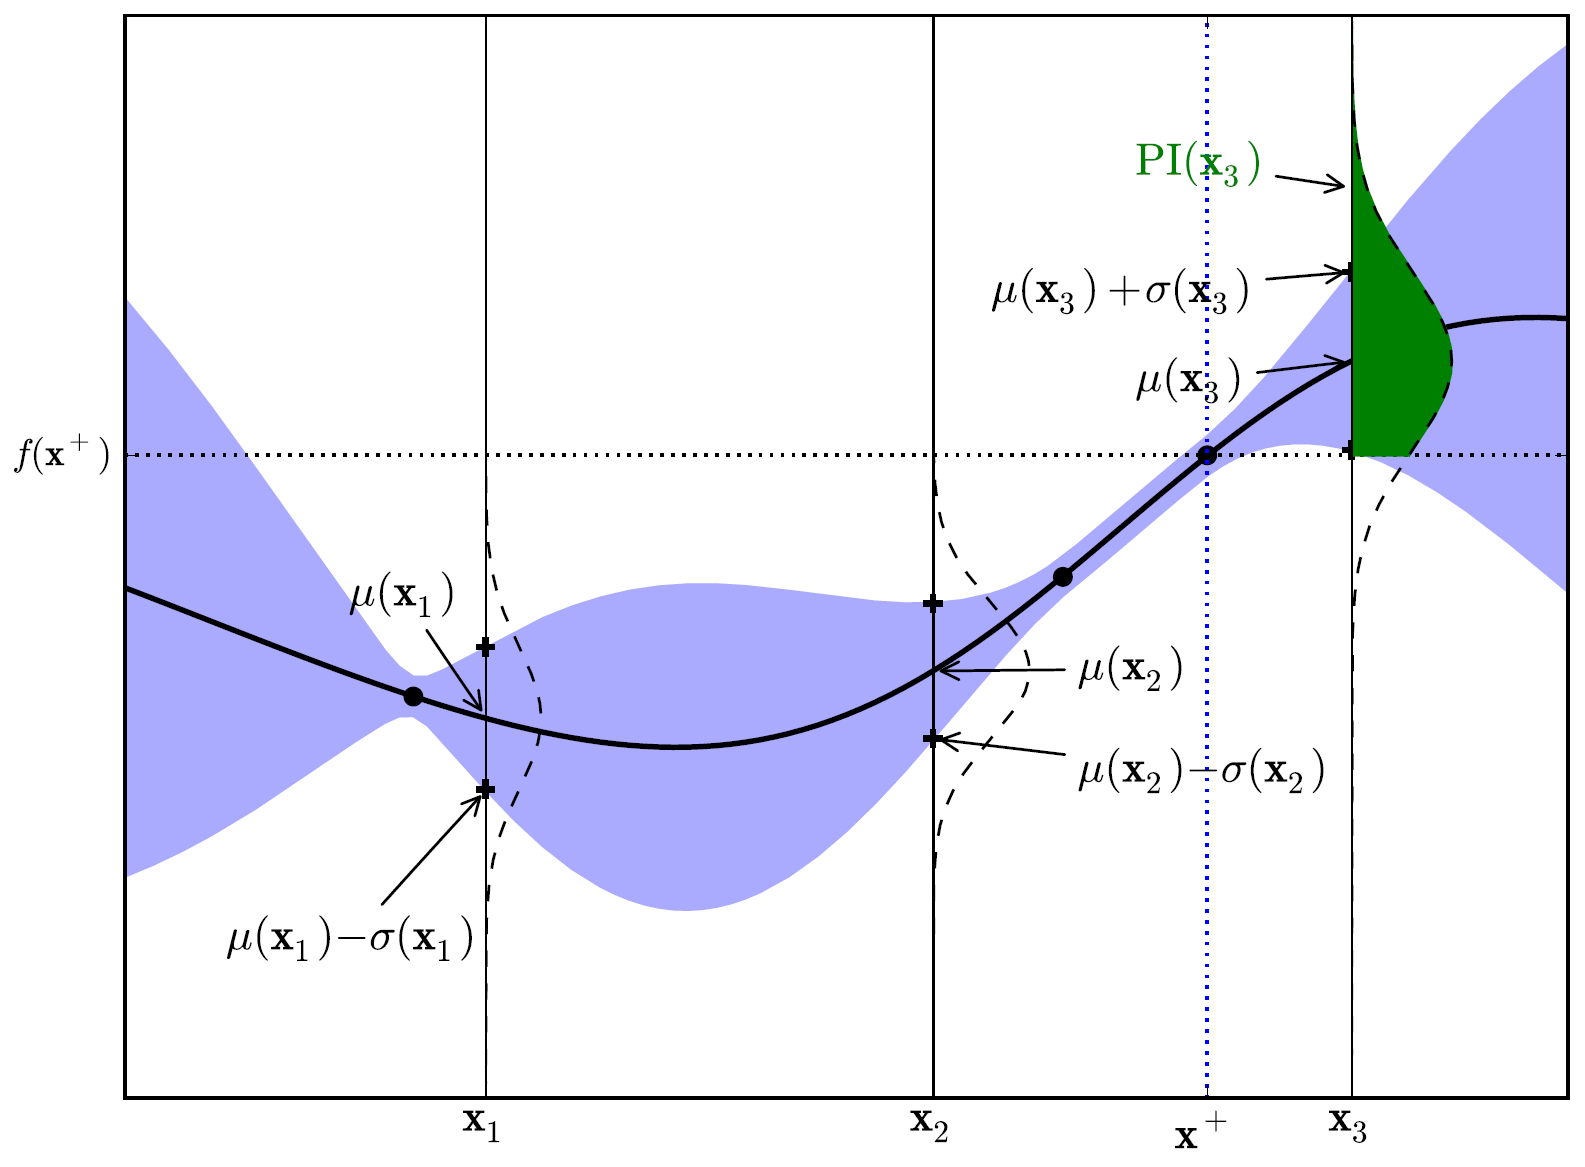
\includegraphics[width=0.55\textwidth]{images/Acquisition-PI.png} 

\end{frame}
%%%%%%%%%%%%%%%%%%%%%%%%%%%%%%%%%%%%%%%%%%%%%%%%%%%%%%%%%%%%%%%%%%%%%%%%%

%%%%%%%%%%%%%%%%%%%%%%%%%%%%%%%%%%%%%%%%%%%%%%%%%%%%%%%%%%%%%%%%%%%%%%%%%
\begin{frame}[c,fragile]{Expected Improvement}

\begin{itemize}
\vspace*{-0.2cm}
  \item Like probability of improvement, but also takes into account the \alert{magnitude} of the improvement.
  \item Define the improvement at a point $\conf$ as:\\
\vspace*{-0.2cm}
  \begin{equation}
  \nonumber{}I(\conf) = \max (f(\conf) - f(\conf^+), 0)
  \end{equation}
  \pause
\vspace*{-0.4cm}  
  \item Then, we can compute the expectation of this improvement across the predictive distribution
  \begin{eqnarray}
\nonumber{} \mathds{E}[I(x)] = \int_{-\infty}^{\infty} \max (f(\conf) - f(\conf^+), 0) \cdot \norm( f(\conf) ; \mu(\conf), \sigma^2(\conf) )  df(\conf) 
  \end{eqnarray}
  \pause
\vspace*{-0.2cm}
  \item This turns out to have a closed form solution:
  \small
  \begin{eqnarray}
\nonumber{} \mathds{E}[I(x)] = (\mu(\conf) - f^+) \Phi\left( \frac{\mu(\conf) - f(\conf^+)}{\sigma(\conf)} \right)  + \sigma(\conf) \phi \left( \frac{\mu(\conf) - f(\conf^+)}{\sigma(\conf)} \right)
  \end{eqnarray}
\end{itemize}

\end{frame}
%%%%%%%%%%%%%%%%%%%%%%%%%%%%%%%%%%%%%%%%%%%%%%%%%%%%%%%%%%%%%%%%%%%%%%%%%

%%%%%%%%%%%%%%%%%%%%%%%%%%%%%%%%%%%%%%%%%%%%%%%%%%%%%%%%%%%%%%%%%%%%%%%%%
\begin{frame}[c,fragile]{Upper Confidence Bound}
\begin{itemize}
\vspace*{-0.2cm}
  \item UCB$(\conf) = \mu(\conf) + \kappa\sigma(\conf)$, with exploration parameter $\kappa$
\end{itemize}
\vspace*{-0.2cm}  
\centering
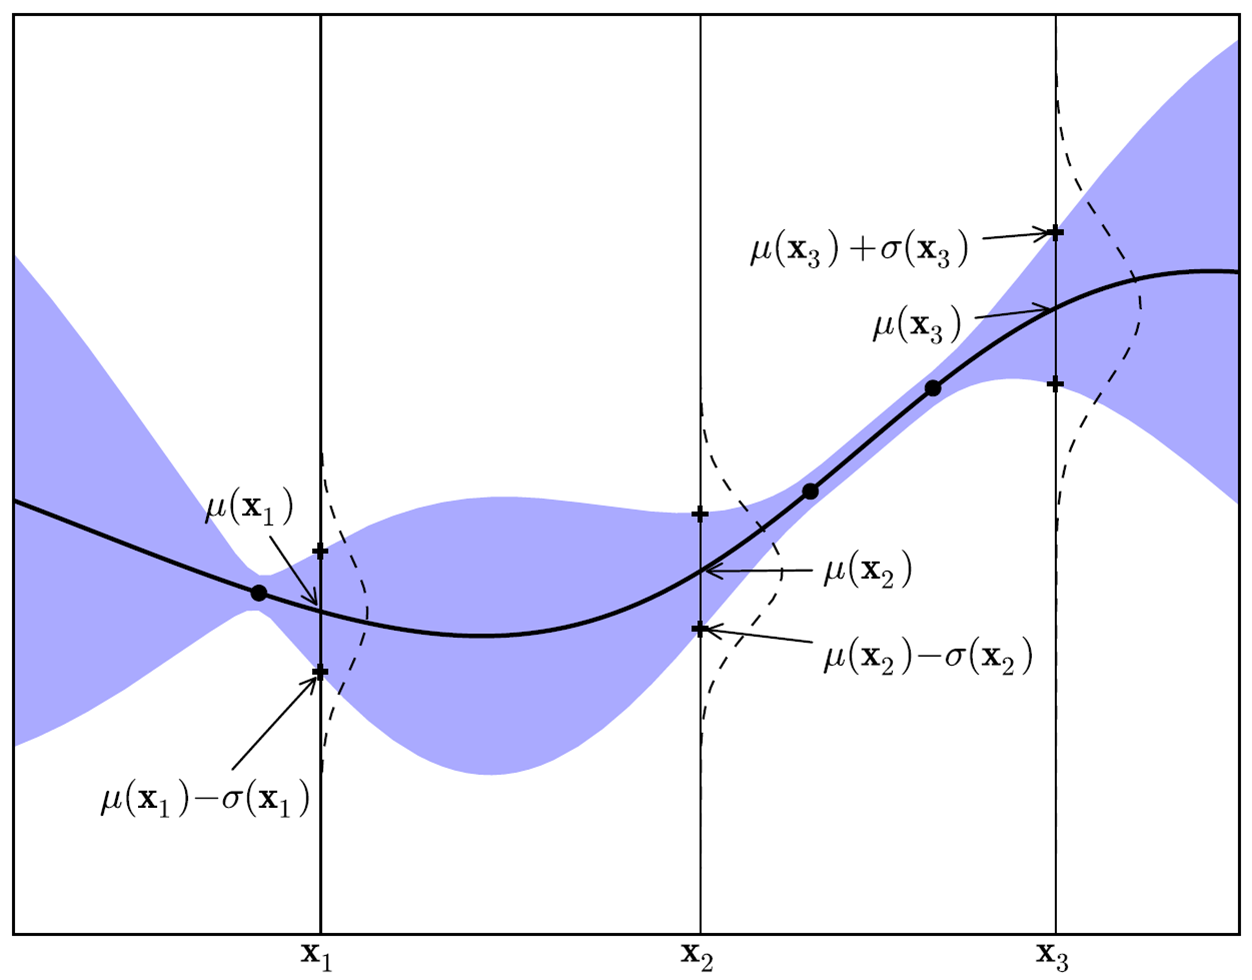
\includegraphics[width=0.55\textwidth]{images/Acquisition-UCB.png} 
\vspace*{0.2cm}  
\begin{itemize}
\item Which point would we pick next with UCB and $\kappa = 1$? \hands
\pause
 \item GP-UCB$(\conf) = \mu(\conf) + \sqrt{\beta_t} \sigma(\conf)$, with $\beta_t$ \alert{increasing} over time\\
 \lit{Srinivas et al. 2009}
\end{itemize}

\end{frame}
%%%%%%%%%%%%%%%%%%%%%%%%%%%%%%%%%%%%%%%%%%%%%%%%%%%%%%%%%%%%%%%%%%%%%%%%%
%%%%%%%%%%%%%%%%%%%%%%%%%%%%%%%%%%%%%%%%%%%%%%%%%%%%%%%%%%%%%%%%%%%%%%%%%
\begin{frame}[c,fragile]{Entropy Search~\litw{Hennig and Schuler 2012}}

\begin{itemize}
	\item Idea: Learn the probability that $x$ is the minimum
\end{itemize}

$$
p_{\text{min}}(x) = p[x \in \argmin f(x)]
$$

\begin{itemize}
	\item try to minimize the entropy of the estimated $p_\text{min}$ distribution
	\item Parts of the approach
	\begin{enumerate}
		\item Estimate $p(f)$ e.g., using a GP (as before)
		\item Discretize $p_\text{min}$ to some representer points
		\item Approximate $p_\text{min}$ by using monte-carle simulations
		\item The acquisition function basically measures how the entropy of $p_\text{min}$ is reduced if we would a new observations
		\begin{itemize}
			\item relates to gaining more information where the optimum is
		\end{itemize}
	\end{enumerate}
	\pause
	\item Remark: This approach does not necessarily samples at the peak of $p_\text{min}$;\\
	You have to trust your model to obtain the expected best $x$ 
\end{itemize}

\end{frame}
%%%%%%%%%%%%%%%%%%%%%%%%%%%%%%%%%%%%%%%%%%%%%%%%%%%%%%%%%%%%%%%%%%%%%%%%%
%%%%%%%%%%%%%%%%%%%%%%%%%%%%%%%%%%%%%%%%%%%%%%%%%%%%%%%%%%%%%%%%%%%%%%%%%
\section{Practical Considerations}
%----------------------------------------------------------------------
\begin{frame}[c]{Preprocessing Configuration}

\begin{block}{Convert $\conf$ for ML Model}
\begin{itemize}
\item continuous and integer parameter can be directly passed
\begin{itemize}
\item scaled to $[0,1]$
\end{itemize}
\pause
\item categorical parameters should be encoded if necessary
\begin{itemize}
\item e.$\,$g., random forest can handle categorical parameter natively\\
(Not all implementations are able to do it!) 
\item use one-hot encoding if necessary:
\begin{itemize}
	\item add new variable for each possible value $v_i$
	\item set one of these variable to one (depending on the configuration)
\end{itemize}
\end{itemize}
\pause
\item ordinal parameters can be converted to integers or also one-hot encoded
\end{itemize}
\end{block}


\end{frame}
%-----------------------------------------------------------------------
%----------------------------------------------------------------------
\begin{frame}[c]{Preprocessing Configuration (cont'd)}

\begin{block}{Conditional Hyperparameters}
\begin{itemize}
\item Configuration spaces often have a hierarchical structure
\item e.$\,$g., hyperparameter A is only active if heuristic H is used
\pause
\item[$\leadsto$] List of hyperparameter values has missing entries because of inactive hyperparameters
\medskip
\pause
\item Fixes:
\begin{itemize}
\item Impute missing data, e.$\,$g., by default setting
\item Mark these inactive hyperparameters and let the model deal with it\\
e.$\,$g., a random forest could only split on active parameters
\end{itemize}
\end{itemize}
\end{block}

\end{frame}
%-----------------------------------------------------------------------
{\setbeamertemplate{logo}{}
\begin{frame}[c,fragile]{Important Design Dimensions in BO}

\only<1>{
\begin{block}{Transformation of y-values}
	\begin{minipage}{0.6\textwidth}
		\begin{figure}[H]
			\centering
			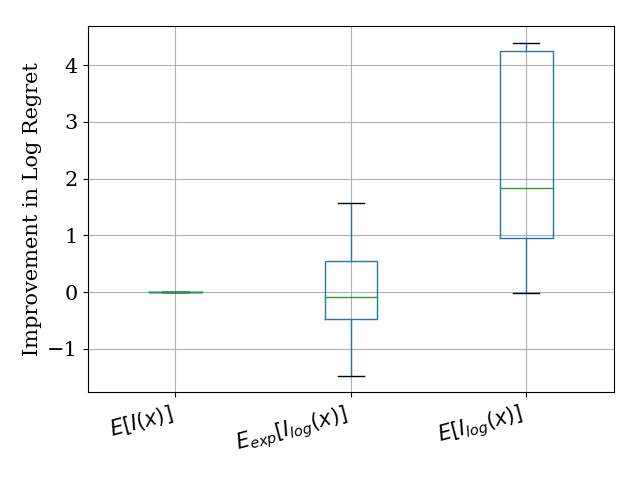
\includegraphics[height=.6\textheight]{images/borf_boxplot_y}
		\end{figure}
	\end{minipage} \hfill
	\begin{minipage}{0.39\textwidth}
		\begin{itemize}
			\item log-transformed values to fit the model and the acquisition function improves performance
			\item less emphasize on large outlier values
			\item focus more on small improvements and less on exploration in unexplored spaces
		\end{itemize}
	\end{minipage}
\end{block}
}

\only<2>{
	\begin{block}{Interleaving Random Points}
		\begin{minipage}{0.6\textwidth}
			\begin{figure}[H]
				\centering
				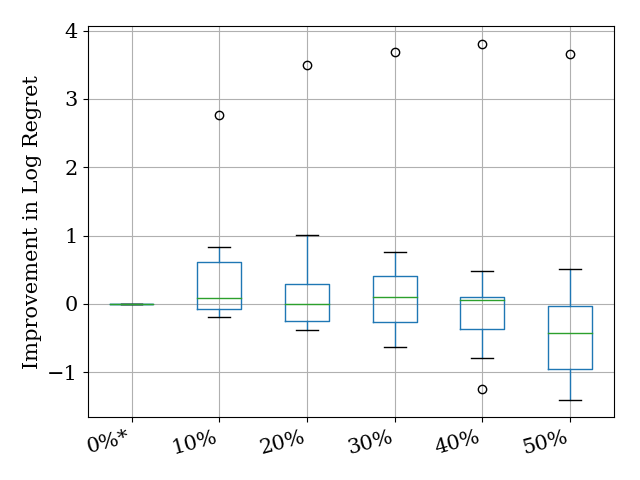
\includegraphics[height=.6\textheight]{images/borf_boxplot_r}
			\end{figure}
		\end{minipage} \hfill
		\begin{minipage}{0.39\textwidth}
			\begin{itemize}
				\item RFs don't extrapolate well
				\item Interpolation between two observations with similar function values leads to
				constant uncertainty estimates
				\item BO with RFs can easily get stuck in local optima
				\item interleave randomly sampled points to escape local optima
			\end{itemize}
		\end{minipage}
	\end{block}
}

\only<3>{
	\begin{block}{Initial Design}
		\begin{minipage}{0.6\textwidth}
			\begin{figure}[H]
				\centering
				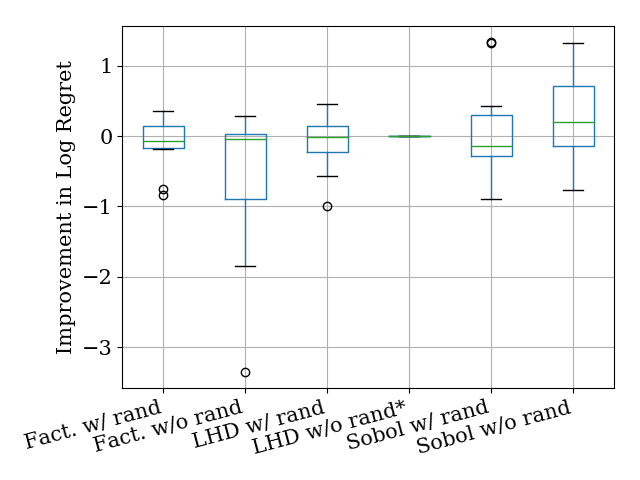
\includegraphics[height=.6\textheight]{images/borf_boxplot_init}
			\end{figure}
		\end{minipage} \hfill
		\begin{minipage}{0.39\textwidth}
			\begin{itemize}
				\item Alternative to exploration via randomly sampled points
				\item explore the space before the actual BO takes place
				\item Pro: will improve the EPM in early iterations
				\item Con: will invest a considerable number of function evaluations without taking the already gathered knowledge into account
			\end{itemize}
		\end{minipage}
	\end{block}
}
\end{frame}
}
%----------------------------------------------------------------------
\begin{frame}[c]{Learning Goals}

After this lecture, you are able to \ldots

\begin{itemize}
	\item explain the \alert{challenges in hyperparameter optimization}
	\item efficiently optimize black box functions via \alert{Bayesian Optimization}
	\item discuss the advantages of different \alert{surrogate models}
	\item explain the idea of \alert{acquisition functions} to trade off exploration and exploitation
	\item consider important design decsisions for BO
\end{itemize}
\end{frame}
%-----------------------------------------------------------------------

%----------------------------------------------------------------------
\begin{frame}[c]{Literature [These are links]}

\begin{itemize}
	\item \lit{\href{https://www.cs.ox.ac.uk/people/nando.defreitas/publications/BayesOptLoop.pdf}{Shahriari et al. 2017. Taking the Human Out of the Loop:
			A Review of Bayesian Optimization}}		
	\item 	
	
\end{itemize}

\end{frame}
%----------------------------------------------------------------------


